\documentclass[10pt, a4paper]{article}
\usepackage[paper=a4paper, left=1.5cm, right=1.5cm, bottom=1.5cm, top=3.5cm]{geometry}
\usepackage[T1]{fontenc}
\usepackage[spanish]{babel}
\usepackage[utf8]{inputenc}
\usepackage{indentfirst}
\usepackage{fancyhdr}
\usepackage{a4wide}
\usepackage[dvipsnames,usenames]{color}
\usepackage{float}
\usepackage{amsmath}
\usepackage{epsfig}
\usepackage{listings}
\usepackage{listingsutf8}
\usepackage{graphicx}
\usepackage{amsfonts}
\usepackage{algpseudocode}
\usepackage[section]{algorithm}
\usepackage{verbatim}
\usepackage{latexsym}
\usepackage{lastpage}
\usepackage[colorlinks=true, linkcolor=blue]{hyperref}
\usepackage{calc}

\newcommand{\f}[1]{\text{#1}}
\newcommand{\real}{\mathbb{R}}
\newcommand{\nat}{\mathbb{N}}
\newcommand{\eme}{\mathcal{M}}
\newcommand{\emeh}{\widehat{\mathcal{M}}}
\newcommand{\ere}{\mathcal{R}}

\sloppy

\setlength{\voffset}{-0.5cm}
\setlength{\hoffset}{0.7cm}
\setlength{\headsep}{0pt}
\setlength{\headheight}{0pt}
\setlength{\oddsidemargin}{-0.7in}
\setlength{\marginparwidth}{-0.5cm}
\setlength{\textwidth}{18cm}
\setlength{\footskip}{2pt}
\setlength{\topmargin}{0in}
\setlength{\textheight}{25cm}
\setlength{\fboxrule}{3pt}

\begin{document}
\thispagestyle{empty}
\begin{center}

\Huge{ \bf{UNIVERSIDAD DE BUENOS AIRES}}
\\
\LARGE{\bf{Facultad de Ciencias Exactas y Naturales}}
\\
\textbf{Departamento de Computaci\'on}
\\
\textbf{M\'etodos Num\'ericos}
\vspace{2.0\baselineskip}
\end{center}


\begin{figure}[h] %[h] Aqui [b] para button [t] para top
\begin{center}

\includegraphics[width=100pt]{./image.jpeg}
\end{center}
\end{figure}
\begin{center}
\vspace*{0.5cm}

\huge{\bf RECUPERATORIO DEL TRABAJO PR\'ACTICO N\'UMERO 2}\\
\huge{Eliminaci\'on del ruido sobre se\~nales unidimensionales y bidimensionales.}
\vspace*{1.6cm}

\end{center}

\LARGE {\textbf{Alumnos:}}\\
\Large{\textsl{Izcovich, Sabrina} $|$ sizcovich@gmail.com}\\
\Large{\textsl{Otero, Fernando} \hspace{0.1cm}$|$ fergabot@gmail.com}\\
\Large{\textsl{Vita, Sebasti\'an} \hspace{0.37cm}$|$ sebastian\_vita@yahoo.com.ar}
\vspace{0.6cm}

\LARGE {\textbf{Palabras Clave:}}\\
\large {PSNR - Señal - Transformada DCT - Ruido}
\vspace*{1cm}

\LARGE{\textbf{Resumen:}}\\
\large {Este trabajo consiste en un an\'alisis sobre diversas señales unidimensionales y bidimensionales con ruido cuyo objetivo es extraer conclusiones en cuanto a la calidad de la señal o imagen recuperada dependiendo de la estrategia utilizada. Para ello, debimos resolver sistemas lineales del tipo $y = Mx$ alterando $y$ de forma tal que, al recuperar $M \tilde{x} = \tilde{y}$, éste resulte con menos ruido. Dicha experimentación fue realizada tanto en vectores como en matrices (extendiendo la transformada DCT a señales de dos dimensiones). Las conclusiones fueron extraídas a partir de estudios de gráficos y experimentaciones explicitadas a continuación.}
\newline
 
\newpage
%Pagina de titulo e indice
\thispagestyle{empty}

\tableofcontents

\newpage

\section{Introducci\'on te\'orica}
Para la realización del estudio de señales, utilizamos los siguientes conceptos:
\begin{itemize}
\item {\textbf{Transformada Discreta del Coseno (DCT):}} Esta herramienta consiste, en el plano continuo, en representar una función en la base de funciones $\mathcal{B}=\{1, \cos(x), \cos(2x),...\}$. En el plano discreto, en cambio, la DCT se corresponde a un cambio de base: cada una de las funciones de la base $\mathcal{B}$ se discretiza en ciertos puntos pasando a ser una base de vectores en $\mathbb{R}^n$ (con n la dimensión del vector o señal a transformar).
\item {\textbf{Frecuencia:}} Es una magnitud que mide el número de repeticiones por unidad de tiempo de cualquier fenómeno o suceso periódico. En nuestro caso, dicha magnitud resultó esencial a la hora de analizar señales pues resultó ser el parámetro de comparación por excelencia.
\item {\textbf{Peak Signal-to-Noise Ratio (PSNR):}} Es una métrica 'perceptual' utilizada como forma para medir la calidad visual de la señal reconstruida \~x. Nos da la forma de medir la calidad de una imagen perturbada a través de su definición:
$$
\mathit{PSNR} = 10 \cdot \log_{10} \left( \frac{\mathit{MAX}^2_x}{\mathit{ECM}} \right)
$$
donde $\mathit{MAX}_x$ define el rango m\'aximo de la se\~nal (en caso de entradas de 8 bits sin signo, ser\'ia 255) y \emph{ECM} es el {\em error cuadr\'atico medio}, definido como:
$ \frac{1}{n} \sum_{i}{(x_{i} - \tilde{x}_{i})^2} $,
donde $n$ es la cantidad de elementos de la se\~nal, $x$ es la se\~nal original y $\tilde{x}$ es la se\~nal recuperada. Cuanto mayor es el PSNR, mayor es la calidad de la imagen.

\item {\textbf{Factorización LU:}} La descomposición LU es una forma de factorización de una matriz como el producto de una matriz triangular inferior y una superior. Dicha descomposición se usa en el análisis numérico para resolver sistemas de ecuaciones más eficientes o encontrar las matrices inversas.

\section{Desarrollo}

\large{\textbf{An\'alisis previo:}}
En primer lugar, es necesario explicitar las variaciones entre ruidos de imagen y de sonido:\newline
\begin{itemize}
\item Las señales sonoras recibidas por los sistemas de captura presentan variaciones continuas que pueden ser de dos tipos:\newline
- Variaciones reales de la señal. En general, variaciones de baja frecuencia.\newline
- Variaciones debidas a interferencias (llamadas ruido). Generalmente, son de alta frecuencia y se eliminan mediante filtrado. Esto es lo que utilizaremos a lo largo de nuestra experimentación.\newline

\item Las señales bidimensionales, en el caso de las imágenes, tienen tipos de ruido que consisten en variaciones que afectan el brillo y/o el color de las mismas. Los tipos de ruido posibles pueden ser, por ejemplo, el Ruido Impulsional en el que ciertos píxeles toman el valor de blanco o negro de forma aleatoria sin tener relación con los píxeles circundantes.\newline
Otro tipo de ruido a considerar es el ruido Gaussiano. Dicho ruido sigue una distribución normal, llamada también distribución Gaussiana, afectando el valor de cada píxel que conforma la imagen.
\end{itemize}

En este trabajo práctico, el objetivo es eliminar el ruido sobre una señal ruidosa $x\in\real^{n}$. Para ello debimos considerar distintas estrategias tanto para agregar como para quitar el ruido de manera tal que resultara interesante cualquier tipo de análisis posterior a las evaluaciones. En primer lugar, pensamos, por ejemplo, que sería buena idea alterar el brillo de las imágenes (por lo tanto aumentar el valor de cada píxel). Al idealizar dicho método, nos percatamos de que la saturación podría llevar a la no recuperación de la imagen original dado que dicho efecto puede generar monotonía en la imagen una vez que se alcanza cierto valor de blanco. Luego, decidimos descartar esta idea.
\newline
Por otro lado, también en el caso de imágenes, se nos ocurrió agregar ruido con el método de ruido impulsivo (conocido también como 'sal y pimienta'). La dificultad se presentaba a la hora de recuperar la imagen ya que no resultaba evidente la manipulación de la misma considerando que los píxeles ruidosos no tiene relación alguna con los píxeles circundantes. Estudiamos la opción de crear un programa que analizara píxel a píxel y que fuera reemplazando cada valor por el promedio de los píxeles circundantes al píxel en cuestión. Dicho programa resultaba acertado para cumplir el objetivo pero las predicciones eran evidentes y no pensamos que fuera una manera apropiada para obtener resultados inesperados e interesantes de los que hubiera que explicar su procedencia.\newline
\newline
Luego de dichos análisis, nos decidimos por los métodos que nos resultaron más interesantes para extraer conclusiones relevantes: \newline
\newline
\large{\textbf{Agregado de ruido:}}\newline
En primer lugar, decidimos agregar ruido de dos maneras distintas: con Ruido Aditivo y Ruido Multiplicativo. De esta manera, pensamos en tomar vectores/matrices $random$ y sumarlas/multiplicarlas a nuestras matrices a alterar. Debido a que decidimos evaluar nuestros resultados en función de la cantidad de ruido agregado, nos percatamos de que el hecho de sumar o multiplicar ruido no variaba los resultados dado que en cada caso nos encargamos de especificar el rango entre el que éste se encontraría. Luego, decidimos utilizar únicamente Ruido Aditivo para realizar nuestro análisis.\newline
 Con el fin de no perder la señal original para poder recuperarla a futuro, utilizamos 60 como $random$ máximo (usado para sumar ruido). De esta manera, nos aseguramos de que las señales no se distorsionaran de tal manera que nos resultaran inservibles para su recuperación. Los ruidos generados se mantuvieron en los siguientes intervalos: \newline
 \begin{itemize}
 \item \center{[-1, 1]}
 \item \center{[-5, 5]}
 \item \center{[-15, 15]}
 \item \center{[-30, 30]}
 \item \center{[-50, 50]}
 \item \center{[-60, 60]}
 \end{itemize}
 
Una vez obtenidos los vectores/matrices, nos limitamos a realizar las operaciones básicas necesarias para sumarlas y obtener una nueva señal con ruido.\newline
\newline
\large{\textbf{Eliminación del ruido:}}\newline
Para ambos tipos de señal, tanto unidimensional como bidimensional, utilizamos el método del valor umbral. Dicho método consiste en la segmentación gráfica de ciertos valores que no aportan datos significativos y cuya eliminación no genera la pérdida de información de la señal.\newline
\newline
En el caso de la señal unidimensional, dicha herramienta resulta ser el nivel de presión sonora con la mínima intensidad necesaria para que un sujeto lo detecte. A partir de ella, eliminamos la señal (igualándola a 0) que supera su valor. De esta manera, se consigue eliminar ruido poco perceptible por el oído humano pero molesto a la hora de escuchar una señal sonora o de visualizar una imagen. Dicho método mantiene las frecuencias altas que resultan ser las más apreciables por el oído humano. \newline
\newline
Por otro lado, en el caso de la señal bidimensional, la idea del umbral se basa en distinguir en una imagen los objetos del fondo de los objetos del primer plano. Dichos elementos de la imagen se distinguen en el gráfico de la señal a través de los picos que presenta. Al segmentar dicho gráfico, los cambios no deberían ser demasiado significativos dado que lo que genera el umbral es la disminución del valor de ciertos píxeles. Esto afecta a la calidad de la imagen sin la pérdida del objeto ni su entorno.\newline
\newline
Teniendo en cuenta la frecuencia de la señal, podemos afirmar que el ruido es oscilatorio y se relaciona con los valores más altos de la transformada. Por lo tanto, cuando borro el ruido mirando la frecuencia asumo que la señal original no tiene muchos saltos y que el ruido se acierta con saltos muy chiquitos por lo que conviene quedarse con los grandes que me van a dar la intensidad. La señal queda casi igual pues el ruido queda captado por los grandes valores.\newline
Los valores elegidos para el umbral fueron considerados manualmente de acuerdo al gráfico de cada señal particular.

\begin{figure}[H] %[h] Aqui [b] para button [t] para top
\begin{center}
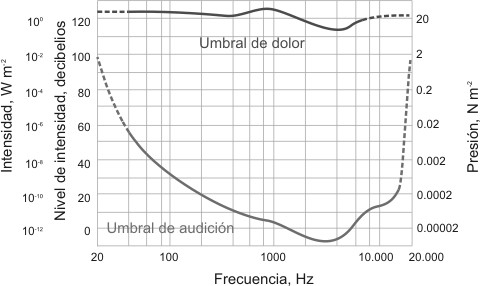
\includegraphics[width=350pt]{./umbrales.jpg}
\caption[h]{Umbral aplicado a ondas sonoras con respecto a la presión y nivel de intensidad.}
\end{center}
\end{figure}

Por otro lado, la otra manera de eliminar el ruido que tuvimos en cuenta fue una idea basada en la {\textbf{Eliminación de frecuencias altas (interferencias) mediante filtrado de la señal}}. Tal como lo explicita el nombre, procedimos a disminuir las frecuencias altas de la señal. Dicho método se basa en los ecualizadores que filtran, atenúan o eliminan frecuencias que molestan, ruidos o interferencias que se mezclan con el sonido. Debido a que, por lo general, los problemas ocurren en un rango determinado de frecuencias, este tipo de método nos pareció adecuado para quitar el ruido. Del mismo modo, pensamos que podría ser interesante aplicarlo a imágenes pues nos interesó experimentar en qué afectaría dicha aplicación en una señal bidimensional.
\newline

\begin{figure}[H] %[h] Aqui [b] para button [t] para top
\begin{center}
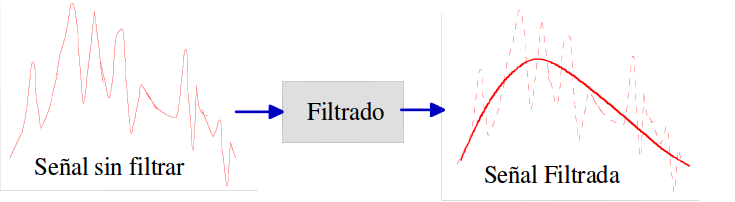
\includegraphics[width=350pt]{./eliminar_frecuencias.png}
\caption[H]{Eliminación de frecuencias altas (interferencias) mediante filtrado de la señal.}
\end{center}
\end{figure}
Un problema hallado en dicho procedimiento fue que, como consecuencia del muestreo de un sistema pueden crearse nuevas frecuencias inexistentes en la señal original, es decir frecuencias que no corresponden ni al ruido ni a la propia señal.\newline

Considerando únicamente los métodos de eliminación del ruido, los resultados esperados al recuperar las señales eran gráficos cercanos a los originales dado que las alteraciones realizadas al agregarlo no debían otorgar diferencias extremas en los valores dados. Por lo tanto, el ruido esperado debía ser fácilmente perceptible pero no debía cambiar la señal de manera rotunda simplificando la eliminación del mismo.\newline
\newline
Nuestro resultado esperado al recuperar la señal con el Método del Valor Umbral era que éste fuera muy similar a la señal original dado que esto fue lo ocurrido en los ejemplos probados en clase. En el caso de la eliminación de frecuencias altas, nuestro resultado esperado fue la recuperación de señales ligeramente más monótonas que las originales dado que los picos de mayor frecuencia habían sido reducidos. De todos modos, lo que esperamos encontrar fueron objetos más nítidos (en el caso de la imagen) y sonidos más puros dado que las frecuencias mayores son las más notorias por lo que el ruido es más evidente en ellas, buscando mimetizarlo con la imagen original.\newline

\large{\textbf{Implementaci\'on:}}
El paso siguiente consistió en programar en C++ los métodos de eliminación y agregado de ruido utilizadas, la funci\'on de la Transformada Discreta del Coseno, el PSNR y el programa para realizar las operaciones necesarias dado un archivo de texto con la cantidad de datos en la primera línea y los propios datos ASCII en la segunda. Del mismo modo, implementamos la factorización LU que nos permite reconstruir la señal de manera eficiente. Para implementar con matrices decidimos utilizar punteros a punteros dado que creamos nuestra matriz de forma dinámica y C++ no acepta que una función reciba una matriz con dimensiones desconocidas.\newline
 
El $main.cpp$ consisti\'o en un men\'u necesario para procesar los archivos de texto que ser\'ian, m\'as tarde, utilizados por las funciones para resolver la DCT y proseguir con la modificación de la señal. Para realizarlo, nos limitamos a utilizar herramientas conocidas (if, while, etc.) y $printf$'s.\newline
En $tcd.cpp$, escribimos las f\'ormulas utilizadas a lo largo del trabajo pr\'actico. Tanto la funci\'on principal para hallar la DCT, el PSNR, como las funciones utilizadas para agregar y eliminar ruido como también las que nos permitieron volver a la señal original recuperada. Para que dichas f\'ormulas fueran legibles, utilizamos los vectores que se descomponen de la matriz $\eme$ para realizar las operaciones necesarias y luego terminar por unirlas correctamente. \newline

\large{\textbf{Modo de uso del programa:}} 
Nuestro programa corre en Windows 7 y Ubuntu. Para compilarlo, recomendamos usar g++. Para ejecutarlo es necesario compilar $tcd.cpp$ y luego, $main.cpp$. Luego, se debe abrir el ejecutable del main.\newline Una vez abierta la interfaz del programa, se debe añadir el archivo de texto junto con su extensión cuyos valores quieran ser procesados. Luego, debe ser seleccionado el tipo de señal a transformar entre unidimensional y bidimensional. Posteriormente, debe elegirse entre agregar ruido sumando random o agregarlo multiplicando random. Por último, debe seleccionarse la función utilizada para quitar el ruido que utilizará la factorización LU para recuperar de manera aproximada la señal original.\newline

\large{\textbf{Recuperaci\'on de resultados:}} Para verificar la correctitud de nuestro programa comparamos los resultados obtenidos con la solución del mismo proceso realizado en Matlab. De esta manera, corroboramos los algoritmos realizados y descartamos experimentos innecesarios. Al realizar varias iteraciones llegamos a la conclusi\'on de que los resultados de nuestro programa resultaban satisfactorios para la mayor\'ia de las pruebas realizadas.\newline

\section{Resultados}
	
\subsection{Señales unidimensionales}
Para realizar las experimentaciones, utilizamos las señales otorgadas por la cátedra 'dopp1024.txt', 'g450.txt' y 'ramp1234.txt'. En primer lugar, graficamos la Transformada Coseno Discreta de los datos en ASCII de dichos archivos junto con el ruido a agregar. En el plano unidimensional, la aplicación de la Transformada puede ser representada como la multiplicación del vector de datos por la matriz de transformación. En cambio, en el plano bidimensional, los cálculos matriciales dificultan las operaciones. Para una simple visualización de los resultados, elegimos plotear las señales unidimensionales. En cambio, en el caso de las señales bidimensionales, preferimos mostrar su imagen característica para que los resultados obtenidos fueran fácilmente visualizables. Si bien nuestras pruebas fueron realizadas con los 6 intervalos de ruido mencionados anteriormente, elegimos utilizar el ruido en [-30,30] para realizar los gráficos dado que es el ruido medio y los demás se comportan de una manera similar dentro de sus propios rangos. Los gráficos que siguen representan a las dct de las señales unidimensionales originales en el plano de las frecuencias:
\newline

\begin{figure}[H] %[h] Aqui [b] para button [t] para top
\begin{center}
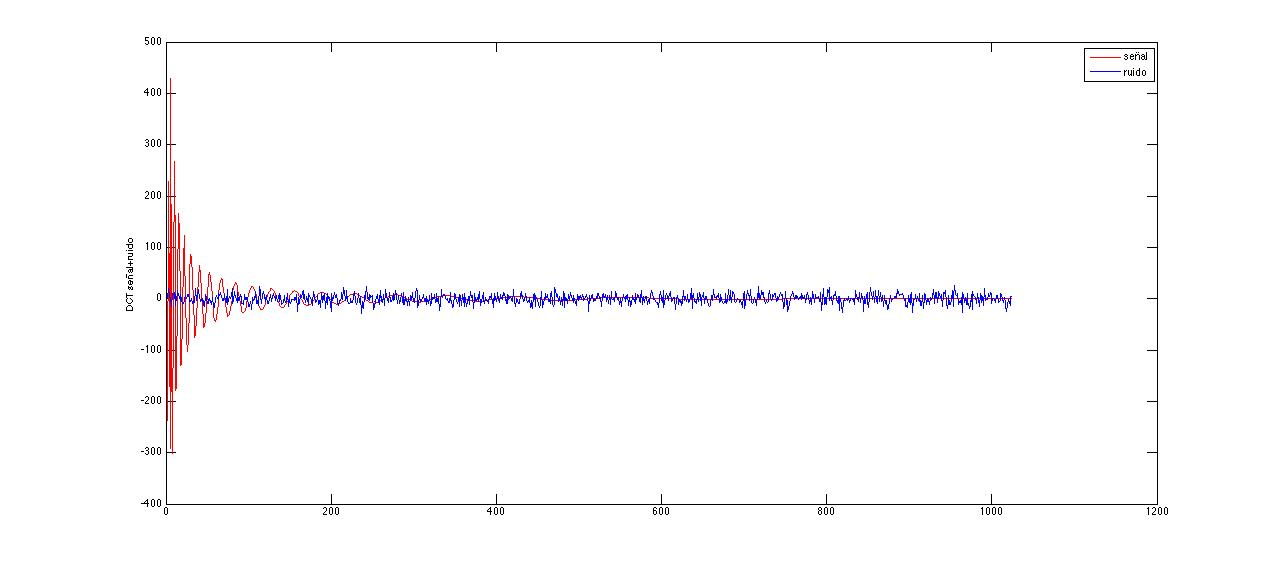
\includegraphics[width=500pt]{./dopp1024_serui.jpg}
\caption[h]{DCT de la señal dopp con 1024 datos y el ruido a agregar en el intervalo [-30, 30].}
\end{center}
\end{figure}

\begin{figure}[H] %[h] Aqui [b] para button [t] para top
\begin{center}
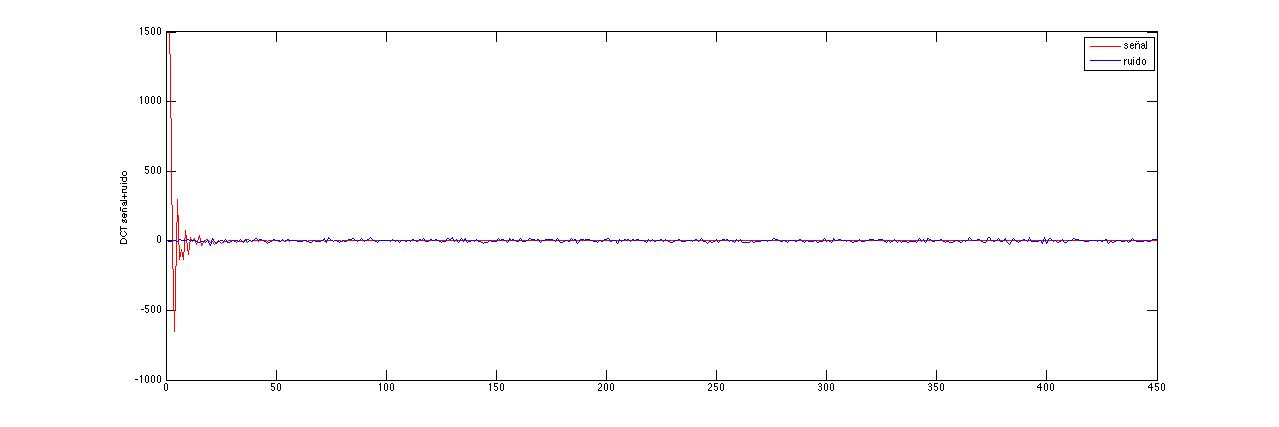
\includegraphics[width=500pt]{./g450_serui.jpg}
\caption[h]{DCT de la señal g con 450 datos y el ruido a agregar en el intervalo [-30, 30].}
\end{center}
\end{figure}

\begin{figure}[H] %[h] Aqui [b] para button [t] para top
\begin{center}
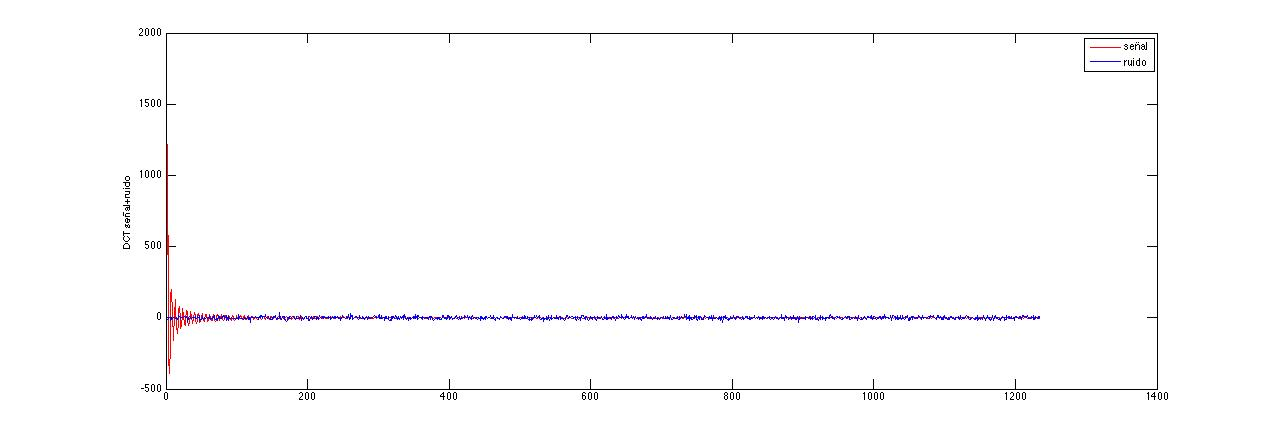
\includegraphics[width=500pt]{./ramp1234_serui.jpg}
\caption[h]{DCT de la señal ramp con 1234 datos y el ruido a agregar en el intervalo [-30, 30].}
\end{center}
\end{figure}

A continuación, proseguimos agregando el ruido. Para realizar ésto, decidimos sumarle los rangos de ruido agregados posteriormente a la señal original. Luego, calculamos la Transformada Coseno Discreta de las señales sumadas. Dado que los gráficos son semejantes a diferencia del alcance del ruido, preferimos dar uno a modo de prueba siendo el resto predecibles. Al igual que en el caso anterior, los gráficos son predecibles por lo que decidimos insertar uno a modo de referencia. Éstos resultaron de la siguiente manera:

\begin{figure}[H] %[h] Aqui [b] para button [t] para top
\begin{center}
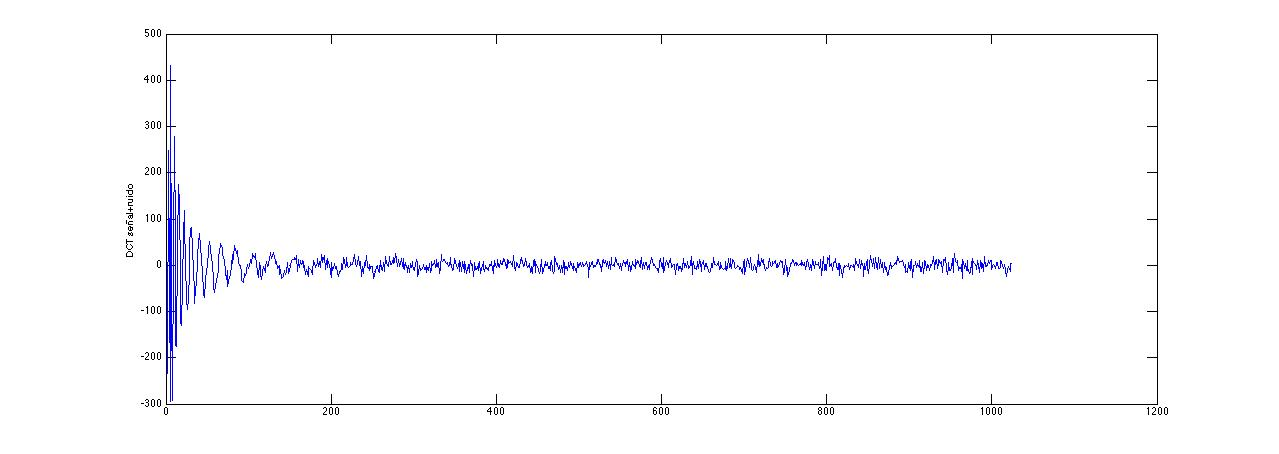
\includegraphics[width=500pt]{./dopp1024_union.jpg}
\caption[h]{DCT de la señal original de dopp con 1024 datos + ruido [-30, 30].}
\end{center}
\end{figure}

\begin{figure}[H] %[h] Aqui [b] para button [t] para top
\begin{center}
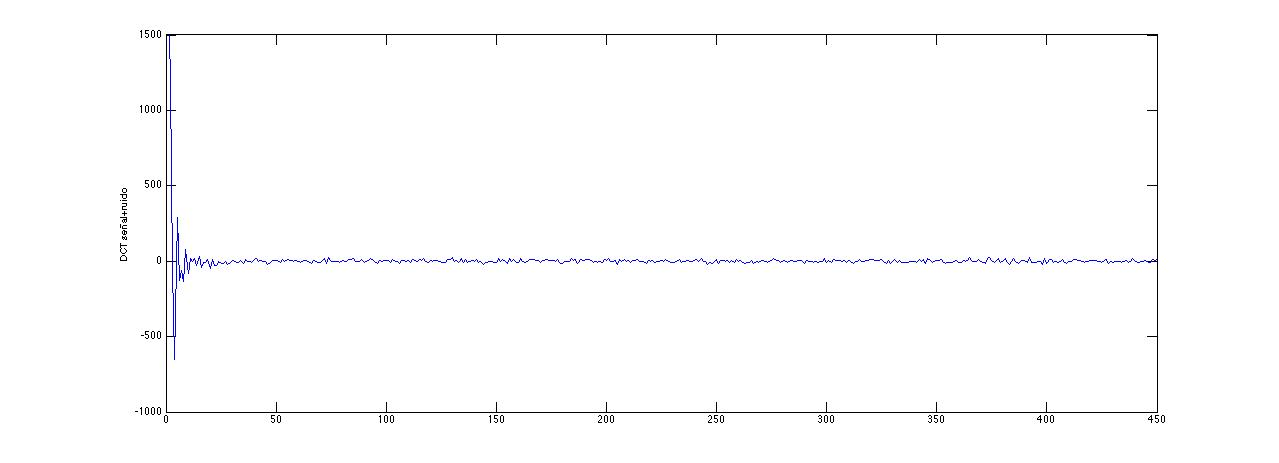
\includegraphics[width=500pt]{./g450_union.jpg}
\caption[h]{DCT de la señal original de g con 450 datos + ruido [-30, 30].}
\end{center}
\end{figure}

\begin{figure}[H] %[h] Aqui [b] para button [t] para top
\begin{center}
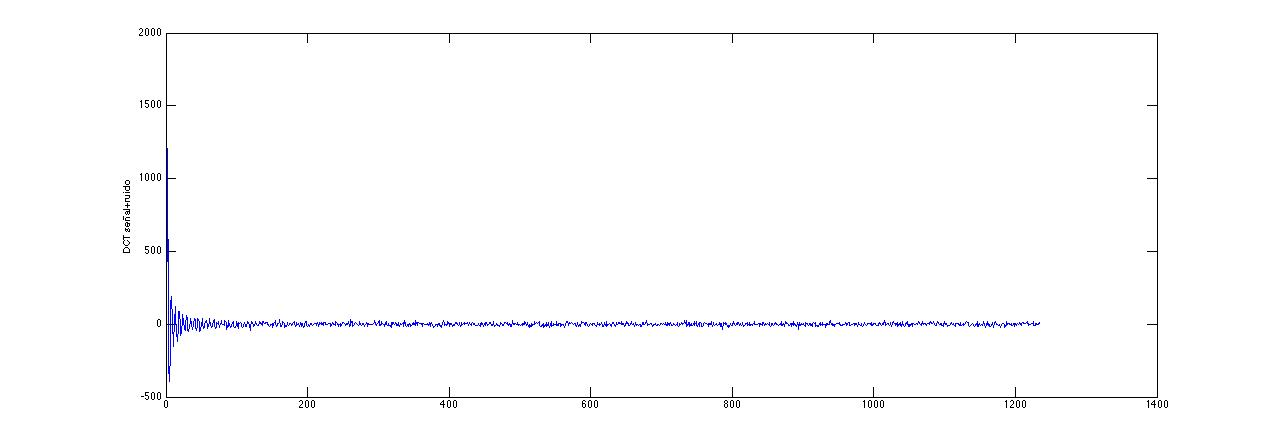
\includegraphics[width=500pt]{./ramp1234_union.jpg}
\caption[h]{DCT de la señal original de ramp con 1234 datos + ruido [-30, 30].}
\end{center}
\end{figure}

Los gráficos fueron alterados en cuanto a longitud para que las frecuencias interesantes fueran visualizables.\newline
\newline

A continuación, le aplicamos la primer función (que aplica el Método del Valor Umbral) a las señales de DCT con ruido agregado sumando random.\newline Luego de diversas pruebas con distintos valores de umbral, nos decidimos por el umbral más coherente para analizar. Por lo tanto, procesamos dichas señales igualando a cero los valores cuyo valor absoluto de su magnitud fuera menor al umbral que fijamos en 5000. En los siguientes gráficos, se puede observar que los valores absolutos mayores a dichas cotas se conservan tal como en la dct de la señal original, en cambio, los valores absolutos menores tienen ahora el valor de 0.


\begin{figure}[H] %[h] Aqui [b] para button [t] para top
\begin{center}
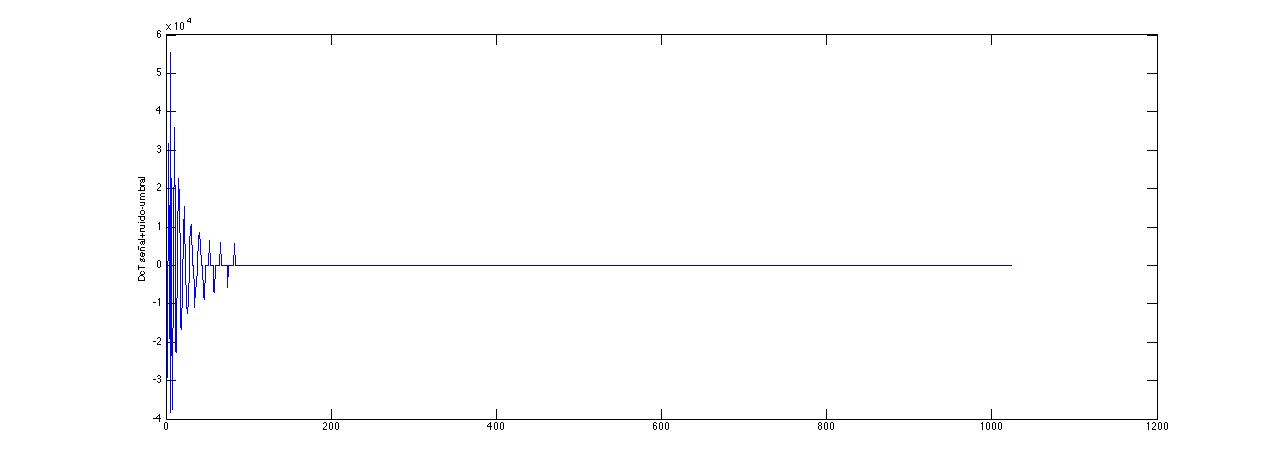
\includegraphics[width=500pt]{./umbral1_dopp1024.jpg}
\caption[h]{DCT de dopp1024 con umbral en 5000.}
\end{center}
\end{figure}


\begin{figure}[H] %[h] Aqui [b] para button [t] para top
\begin{center}
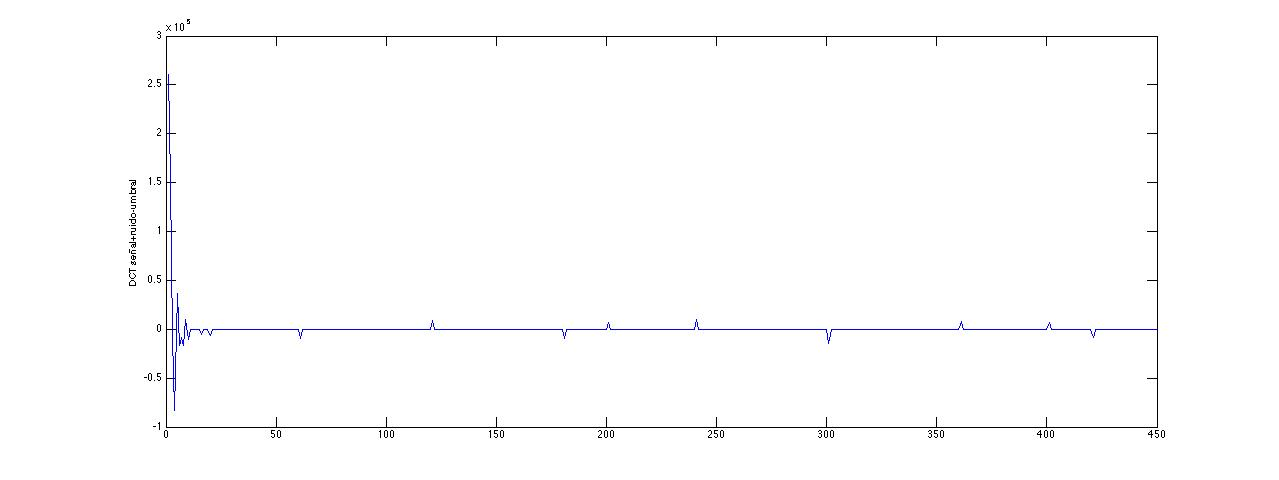
\includegraphics[width=500pt]{./umbral1_g450.jpg}
\caption[h]{DCT de g450 con umbral en 5000.}
\end{center}
\end{figure}


\begin{figure}[H] %[h] Aqui [b] para button [t] para top
\begin{center}
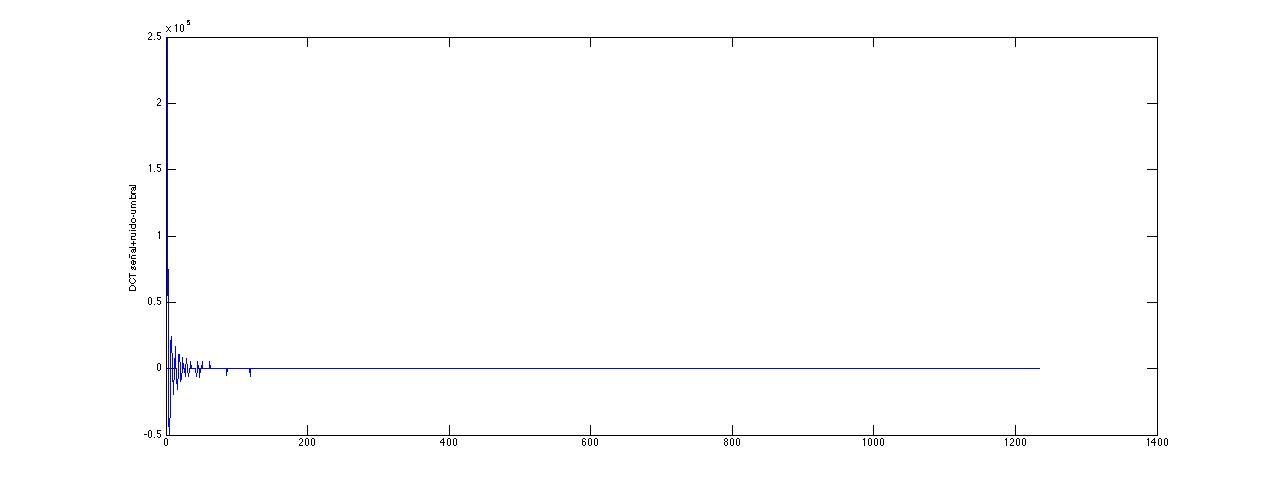
\includegraphics[width=500pt]{./umbral1_ramp1234.jpg}
\caption[h]{DCT de ramp1234 con umbral en 5000.}
\end{center}
\end{figure}

Lo que sigue consistió en aplicar la M correspondiente (para obtener $M*$\~x = \~y) para la vuelta a la señal original. En los gráficos siguientes, se puede ver cómo resultaron las señales en comparación con la señal original para cada rango de ruido.
\begin{itemize}

\item \center{\textbf{\Large{dopp1024}}}

\begin{figure}[H] %[h] Aqui [b] para button [t] para top
\begin{center}
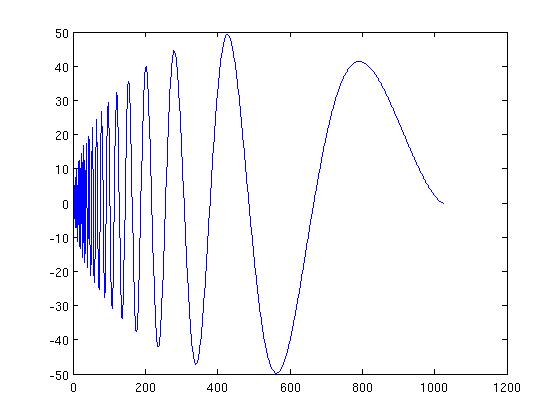
\includegraphics[width=300pt]{./dopp1024.jpg}
\caption[h]{dopp1024 original.}
\end{center}
\end{figure}

\begin{figure}[H] % indico que voy a poner una figura y [h] indica que la posición relativa, tambien puedo usar t = top entre otros.
\hfill
\begin{minipage}[t]{.45\textwidth}
\begin{center}
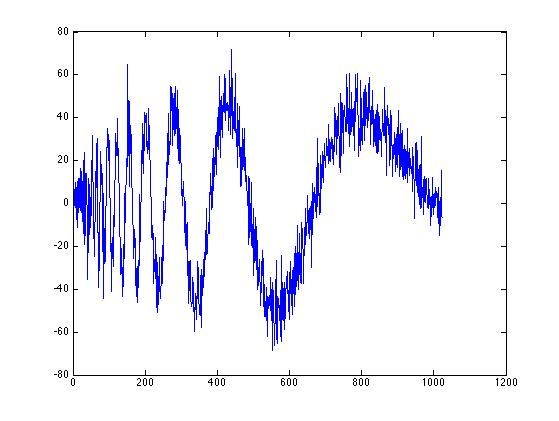
\epsfig{file=dopp1024_recu1000.jpg, scale=0.4} % primera imagen colocada a la izquierda
\caption{DCT de dopp1024 recuperada con un umbral de 1000}
\label{fig-tc1}
\end{center}
\end{minipage}
\hfill
\begin{minipage}[t]{.45\textwidth}
\begin{center}
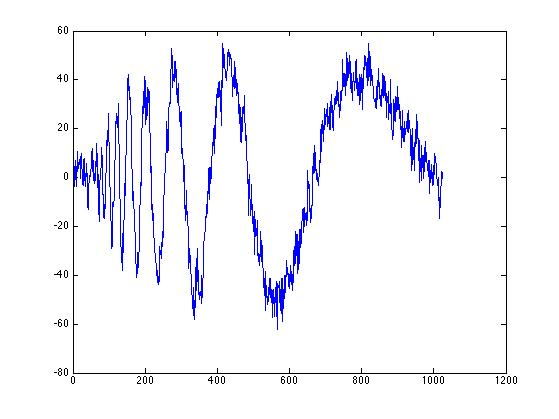
\epsfig{file=dopp1024_recu3000.jpg, scale=0.4} % segunda imagen colocada a la derecha
\caption{DCT de dopp1024 recuperada con un umbral de 3000}
\label{fig-tc2}
\end{center}
\end{minipage}
\hfill
\end{figure} 

\begin{figure}[H] % indico que voy a poner una figura y [h] indica que la posición relativa, tambien puedo usar t = top entre otros.
\hfill
\begin{minipage}[t]{.45\textwidth}
\begin{center}
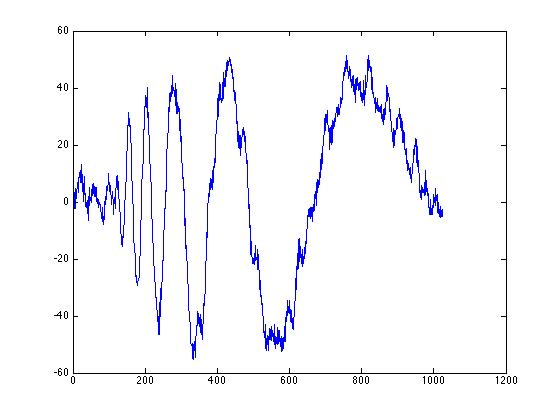
\epsfig{file=dopp1024_recu5000.jpg, scale=0.4} % primera imagen colocada a la izquierda
\caption{DCT de dopp1024 recuperada con un umbral de 5000}
\label{fig-tc1}
\end{center}
\end{minipage}
\hfill
\begin{minipage}[t]{.45\textwidth}
\begin{center}
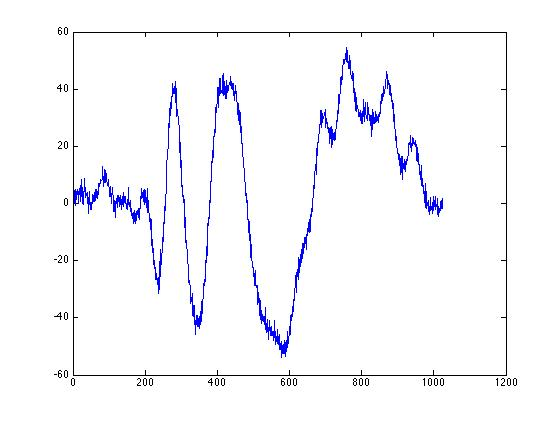
\epsfig{file=dopp1024_recu10000.jpg, scale=0.4} % segunda imagen colocada a la derecha
\caption{DCT de dopp1024 recuperada con un umbral de 10000}
\label{fig-tc2}
\end{center}
\end{minipage}
\hfill
\end{figure} 

\item \center{\textbf{\Large{g450}}}
\begin{figure}[H] %[h] Aqui [b] para button [t] para top
\begin{center}
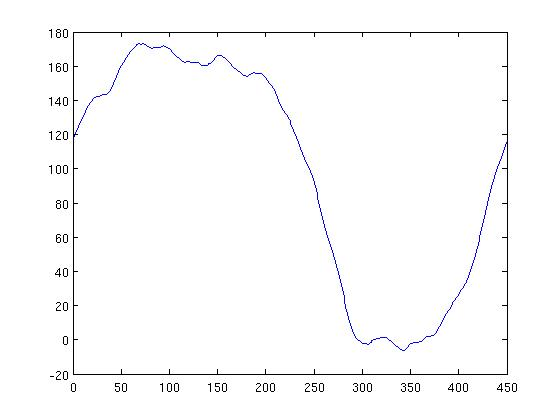
\includegraphics[width=300pt]{./g450.jpg}
\caption[h]{g450 original.}
\end{center}
\end{figure}

\begin{figure}[H] % indico que voy a poner una figura y [h] indica que la posición relativa, tambien puedo usar t = top entre otros.
\hfill
\begin{minipage}[t]{.45\textwidth}
\begin{center}
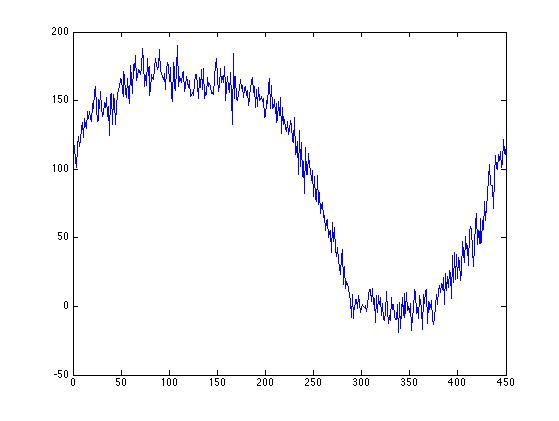
\epsfig{file=g450_recu1000.jpg, scale=0.4} % primera imagen colocada a la izquierda
\caption{DCT de g450 recuperada con un umbral de 1000}
\label{fig-tc1}
\end{center}
\end{minipage}
\hfill
\begin{minipage}[t]{.45\textwidth}
\begin{center}
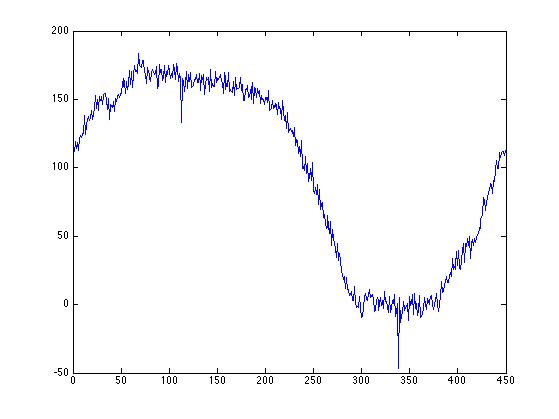
\epsfig{file=g450_recu3000.jpg, scale=0.4} % segunda imagen colocada a la derecha
\caption{DCT de g450 recuperada con un umbral de 3000}
\label{fig-tc2}
\end{center}
\end{minipage}
\hfill
\end{figure} 

\begin{figure}[H] % indico que voy a poner una figura y [h] indica que la posición relativa, tambien puedo usar t = top entre otros.
\hfill
\begin{minipage}[t]{.45\textwidth}
\begin{center}
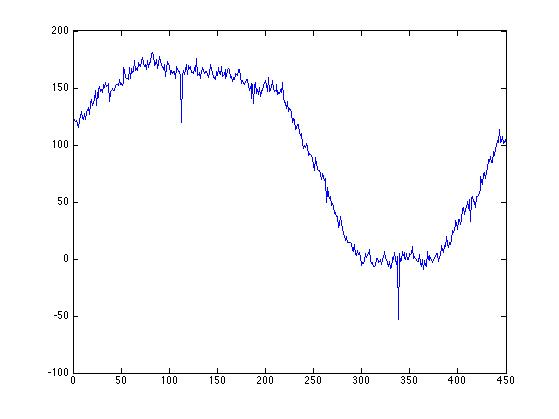
\epsfig{file=g450_recu5000.jpg, scale=0.4} % primera imagen colocada a la izquierda
\caption{DCT de g450 recuperada con un umbral de 5000}
\label{fig-tc1}
\end{center}
\end{minipage}
\hfill
\begin{minipage}[t]{.45\textwidth}
\begin{center}
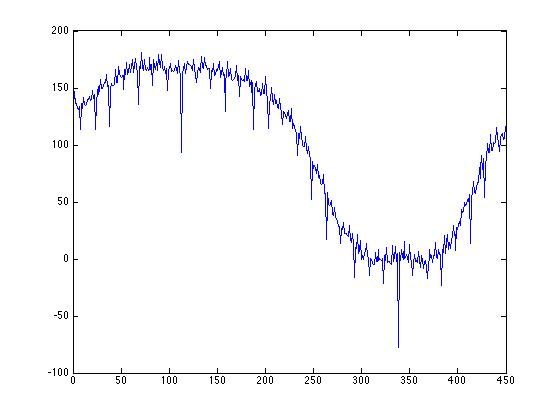
\epsfig{file=g450_recu10000.jpg, scale=0.4} % segunda imagen colocada a la derecha
\caption{DCT de g450 recuperada con un umbral de 10000}
\label{fig-tc2}
\end{center}
\end{minipage}
\hfill
\end{figure} 

\item \center{\textbf{\Large{ramp1234}}}

\begin{figure}[H] %[h] Aqui [b] para button [t] para top
\begin{center}
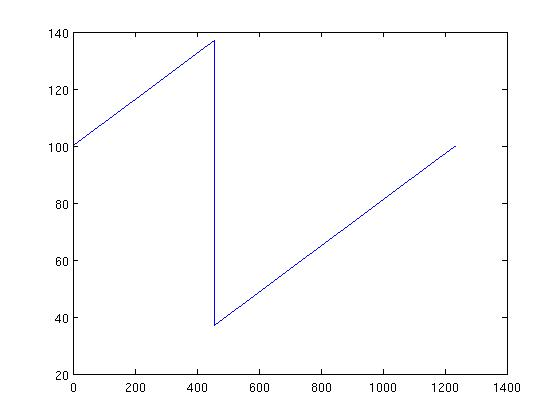
\includegraphics[width=300pt]{./ramp1234.jpg}
\caption[h]{ramp1234 original.}
\end{center}
\end{figure}

\begin{figure}[H] % indico que voy a poner una figura y [h] indica que la posición relativa, tambien puedo usar t = top entre otros.
\hfill
\begin{minipage}[t]{.45\textwidth}
\begin{center}
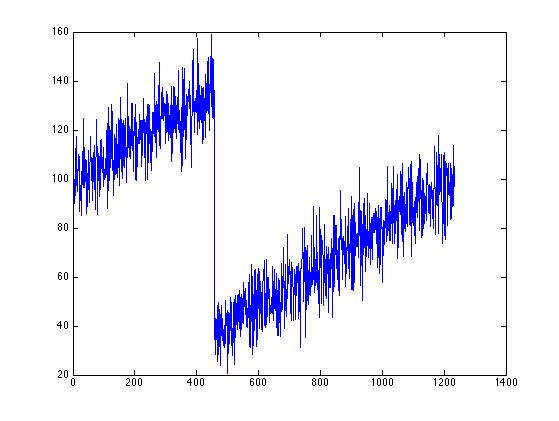
\epsfig{file=ramp1234_recu1000.jpg, scale=0.4} % primera imagen colocada a la izquierda
\caption{DCT de ramp1234 recuperada con un umbral de 1000}
\label{fig-tc1}
\end{center}
\end{minipage}
\hfill
\begin{minipage}[t]{.45\textwidth}
\begin{center}
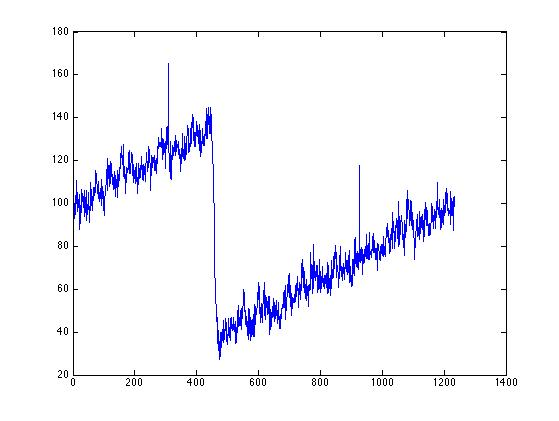
\epsfig{file=ramp1234_recu3000.jpg, scale=0.4} % segunda imagen colocada a la derecha
\caption{DCT de ramp1234 recuperada con un umbral de 3000}
\label{fig-tc2}
\end{center}
\end{minipage}
\hfill
\end{figure} 

\begin{figure}[H] % indico que voy a poner una figura y [h] indica que la posición relativa, tambien puedo usar t = top entre otros.
\hfill
\begin{minipage}[t]{.45\textwidth}
\begin{center}
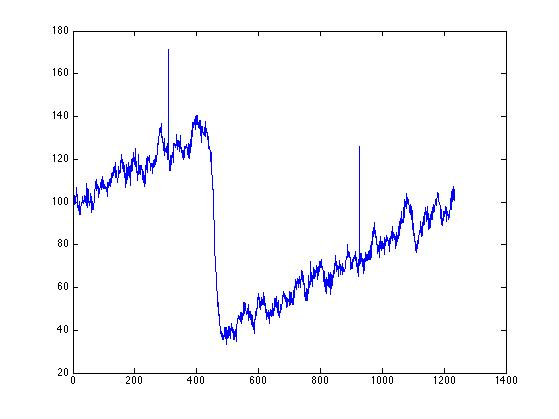
\epsfig{file=ramp1234_recu5000.jpg, scale=0.4} % primera imagen colocada a la izquierda
\caption{DCT de ramp1234 recuperada con un umbral de 5000}
\label{fig-tc1}
\end{center}
\end{minipage}
\hfill
\begin{minipage}[t]{.45\textwidth}
\begin{center}
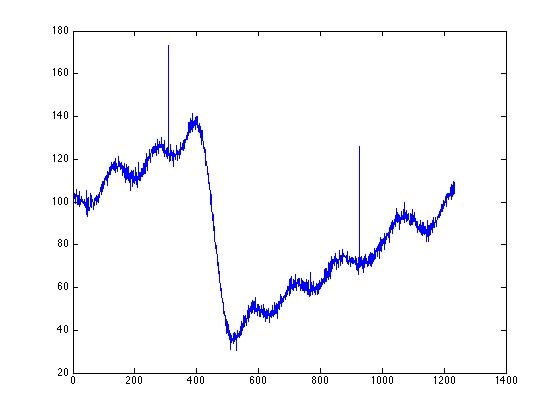
\epsfig{file=ramp1234_recu10000.jpg, scale=0.4} % segunda imagen colocada a la derecha
\caption{DCT de ramp1234 recuperada con un umbral de 10000}
\label{fig-tc2}
\end{center}
\end{minipage}
\hfill
\end{figure} 
\end{itemize}

Luego, recuperamos los valores de los PSNR de acuerdo a la cantidad de ruido agregado para lograr obtener una relación lineal entre la cantidad de ruido agregado y la cantidad de ruido eliminado. Debido a que el PSNR es una métrica perceptual que divide el error cuadrático medio, un resultado grande ($\geq$ 20) expone que las señales evaluadas se parecen. En cambio, si el resultado permanece entre números pequeños (menores que 5) nos dice que las señales no son semejantes. Los resultados obtenidos fueron los siguientes:\newline
 
\begin{figure}[H] %[h] Aqui [b] para button [t] para top
\begin{center}
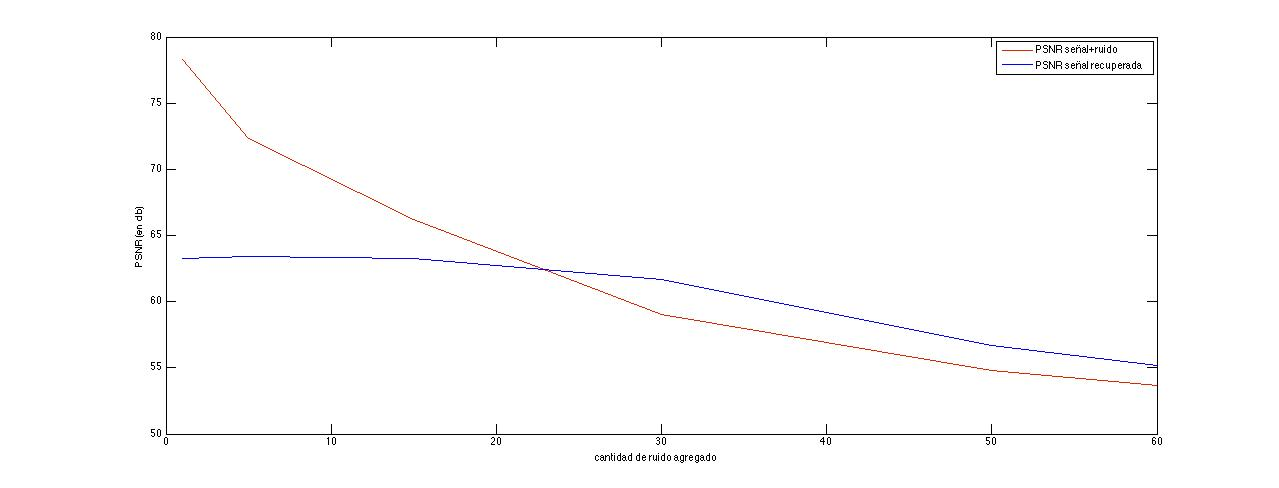
\includegraphics[width=550pt]{./psnr_1024.jpg}
\caption[h]{PSNR de la señal dopp1024+ruido y PSNR de la señal recuperada respecto de la cantidad de ruido agregado.}
\end{center}
\end{figure}

\begin{figure}[H] %[h] Aqui [b] para button [t] para top
\begin{center}
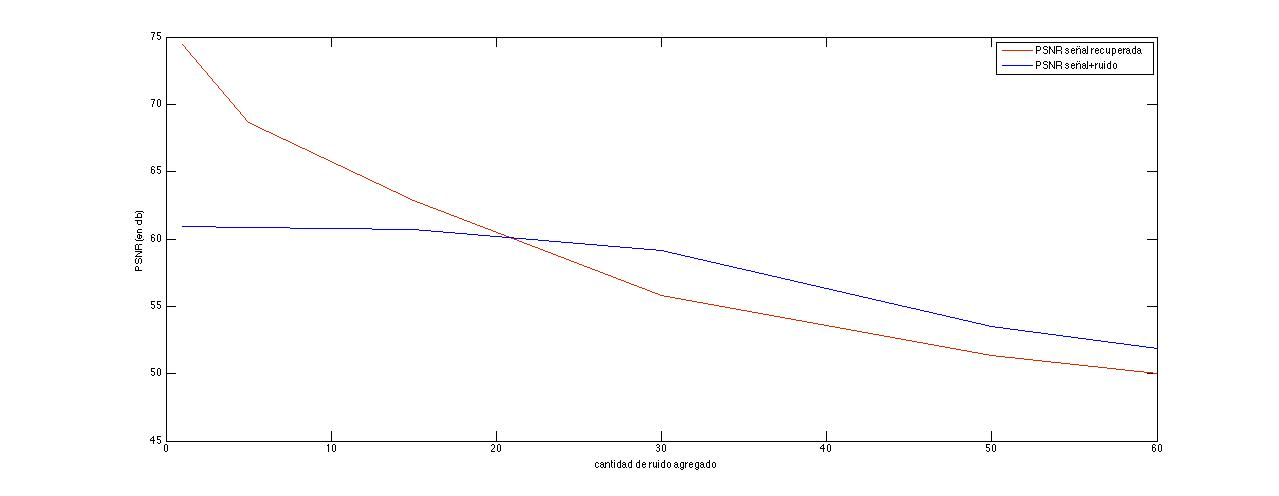
\includegraphics[width=550pt]{./psnr_450.jpg}
\caption[h]{PSNR de la señal g450+ruido y PSNR de la señal recuperada respecto de la cantidad de ruido agregado.}
\end{center}
\end{figure}

\begin{figure}[H] %[h] Aqui [b] para button [t] para top
\begin{center}
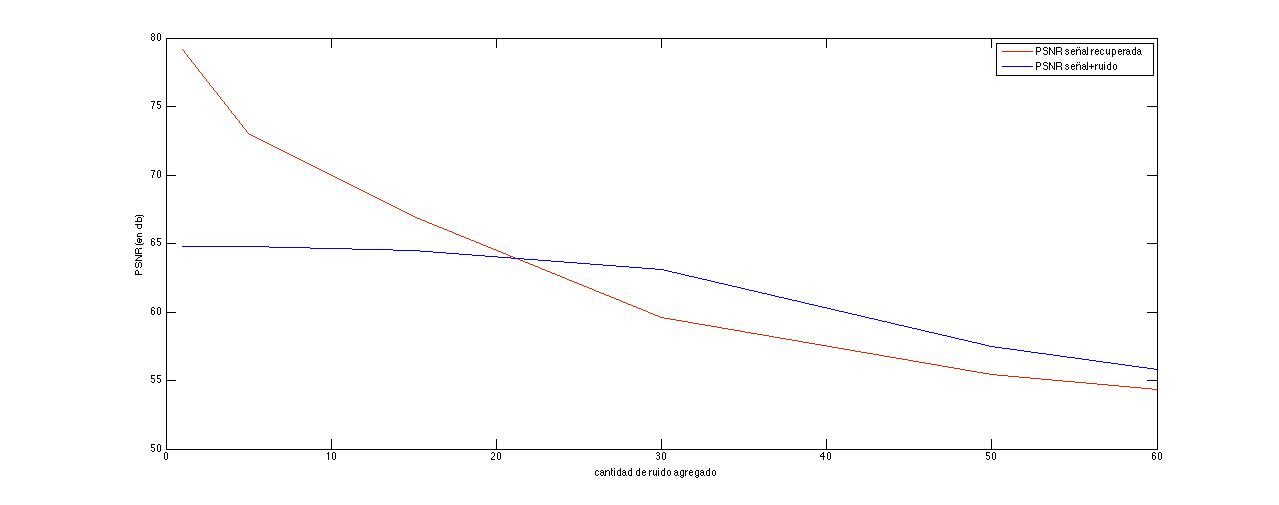
\includegraphics[width=550pt]{./psnr_1234.jpg}
\caption[h]{PSNR de la señal ramp1234+ruido y PSNR de la señal recuperada respecto de la cantidad de ruido agregado.}
\end{center}
\end{figure}


Luego, procedimos aplicando el segundo método 'Eliminación de frecuencias altas mediante filtrado de la señal'. En este caso, debimos evaluar diversos errores a partir de los cuales se reduciría parte de la frecuencia. Las pruebas realizadas consistieron en alternar la cota a partir de la que se reduciría la señal como también el valor que se le restaría a los valores de ésta que superaran dicha cota. Luego de distintas pruebas, notamos que la variación entre la señal con ruido y la señal recuperada no era realmente notoria en la mayoría de los casos. Los resultados obtenidos fueron los siguientes:

\begin{figure}[H] %[h] Aqui [b] para button [t] para top
\begin{center}
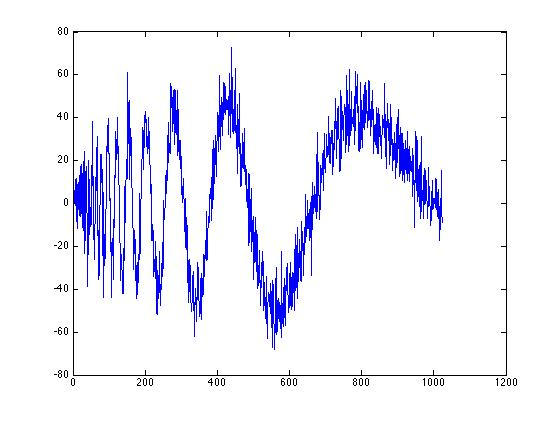
\includegraphics[width=350pt]{./dopp1024_recu_f2.jpg}
\caption[h]{Señal dopp1024 recuperada utilizando una cota de 10000 y reduciendo las frecuencias de 50.}
\end{center}
\end{figure}

\begin{figure}[H] %[h] Aqui [b] para button [t] para top
\begin{center}
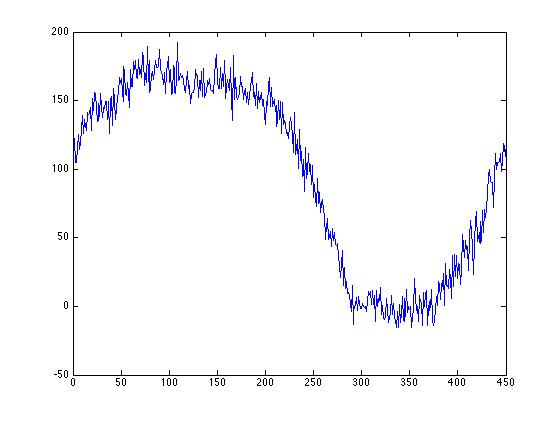
\includegraphics[width=350pt]{./g450_recu_f2.jpg}
\caption[h]{Señal g450 recuperada utilizando una cota de 10000 y reduciendo las frecuencias de 50.}
\end{center}
\end{figure}

\begin{figure}[H] %[h] Aqui [b] para button [t] para top
\begin{center}
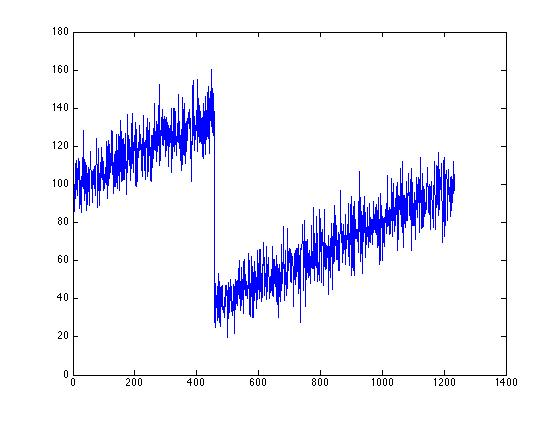
\includegraphics[width=350pt]{./ramp1234_recu_f2.jpg}
\caption[h]{Señal ramp1234 recuperada utilizando una cota de 10000 y reduciendo las frecuencias de 50.}
\end{center}
\end{figure}

Para poder sacar conclusiones de los resultados obtenidos, decidimos realizar un gráfico en el que se pudiera visualizar la variación del PSNR en función de la cantidad de ruido agregado a la señal:

\begin{figure}[H] %[h] Aqui [b] para button [t] para top
\begin{center}
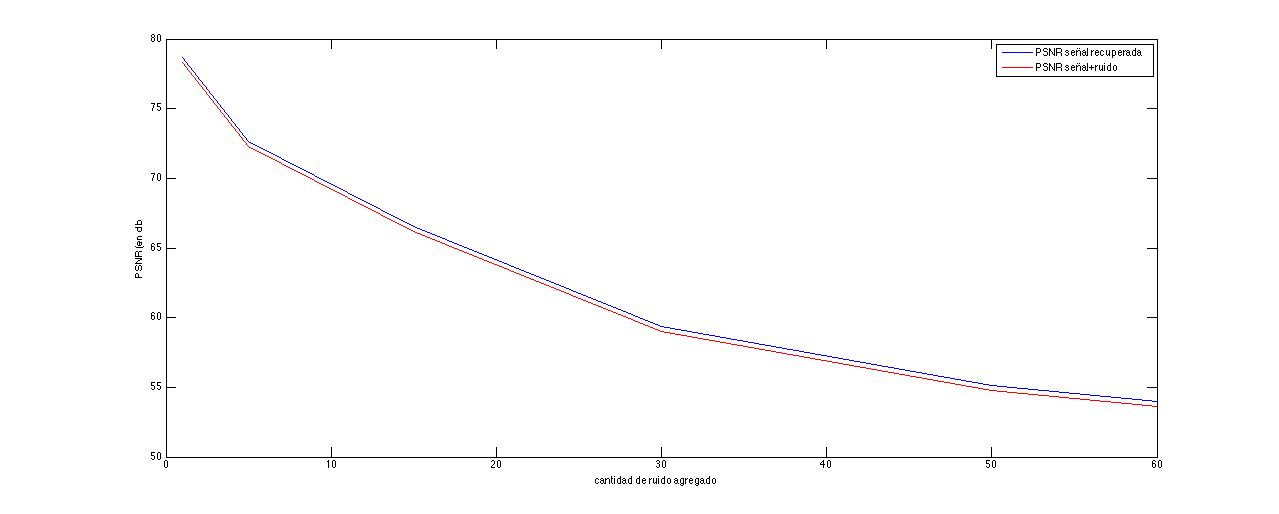
\includegraphics[width=550pt]{./psnr_dopp1024_f2.jpg}
\caption[h]{PSNR de la señal dopp1024+ruido y PSNR de la señal recuperada respecto de la cantidad de ruido agregado.}
\end{center}
\end{figure}

\begin{figure}[H] %[h] Aqui [b] para button [t] para top
\begin{center}
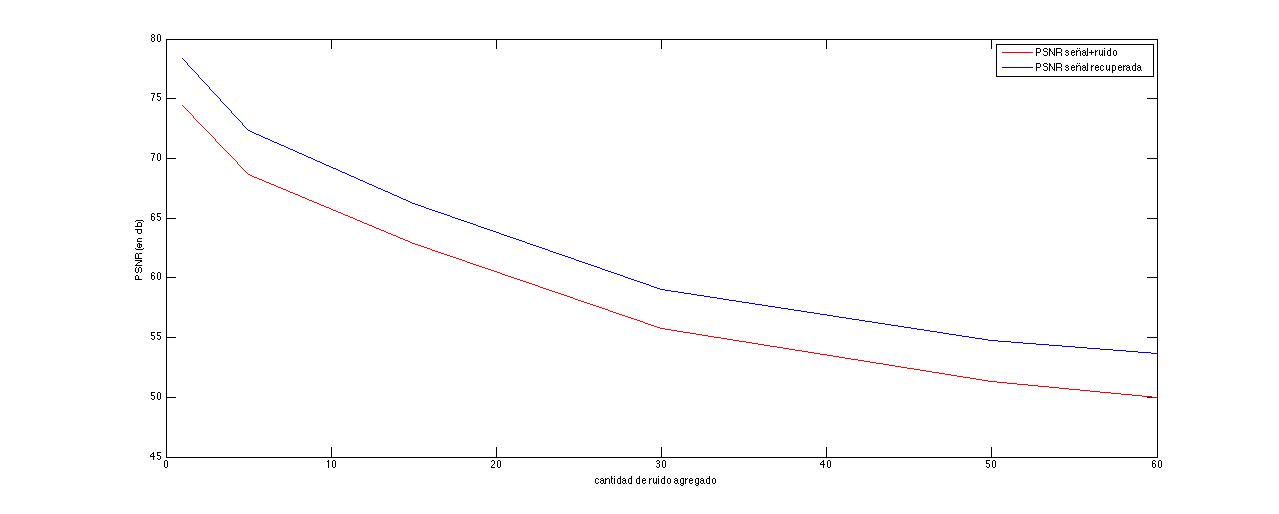
\includegraphics[width=550pt]{./psnr_g450_f2.jpg}
\caption[h]{PSNR de la señal g450+ruido y PSNR de la señal recuperada respecto de la cantidad de ruido agregado.}
\end{center}
\end{figure}

\begin{figure}[H] %[h] Aqui [b] para button [t] para top
\begin{center}
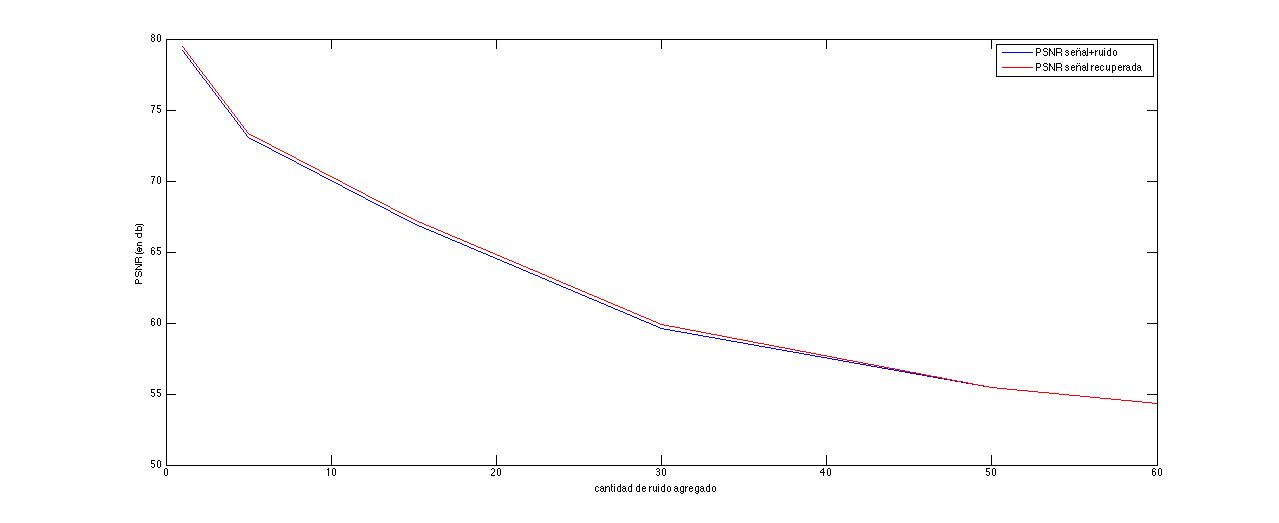
\includegraphics[width=550pt]{./psnr_ramp1234_f2.jpg}
\caption[h]{PSNR de la señal ramp1234+ruido y PSNR de la señal recuperada respecto de la cantidad de ruido agregado.}
\end{center}
\end{figure}

Se puede observar que los PSNR demuestran que el resultado es levemente mejor sin importar la cantidad de ruido agregado. Esto se debe a que al reducir la frecuencia de los valores más presentes en la señal (que es donde más ruido se preserva) la cantidad de ruido se aminora sin importar cuánto sea éste. Si bien este método no resulta eficaz, resulta interesante que, en la gran mayoría de los casos, siempre hay una leve mejoría.

\subsection{Señales bidimensionales}

Para las señales bidimensionales, utilizamos los mismos métodos para quitar el ruido. Primero, nos enfrentamos con la decisión de elegir un umbral que nos diera buenos resultados en la mayor parte de los casos. Para ello probamos, para una abundante combinación de cotas y cantidad de ruido, una enorme cantidad de experiencias. De este modo, se tuvieron en cuenta diferentes ruidos para una misma cota y se realizaron diversas variaciones de cada rango generado aleatoriamente.\newline
El algoritmo utilizado es de la siguiente forma:

\begin{algorithm}[H]
\begin{algorithmic}[1]
\For {cada cota}
   \For {cada ruido}
   	\State {resuelvo sistema con DCT}
   	\State {calculoPSNR} 
   	\Comment{Si el PSNR de la imagen recuperada es mayor que 20 lo guardo}
   	
   \EndFor
   \State{promedio los resultados en los que la imagen mejoró}
   
   \EndFor
   \State{comparo los promedios y me quedo con la cota que mejor dio}
\end{algorithmic}
\end{algorithm}

Las señales bidimensionales utilizadas para la experimentación fueron las siguientes:

\begin{figure}[!htb]
\minipage{0.32\textwidth}
  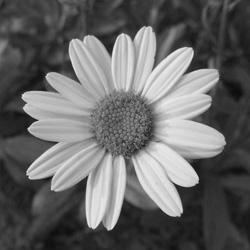
\includegraphics[width=\linewidth]{imagen1.jpg}
  \caption{Imagen 1.}\label{fig:awesome_image1}
\endminipage\hfill
\minipage{0.32\textwidth}
  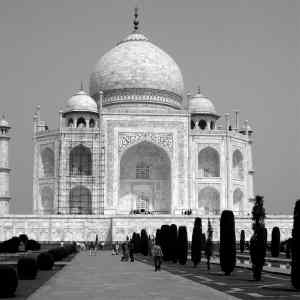
\includegraphics[width=\linewidth]{imagen2.jpg}
  \caption{Imagen 2.}\label{fig:awesome_image2}
\endminipage\hfill
\minipage{0.32\textwidth}%
  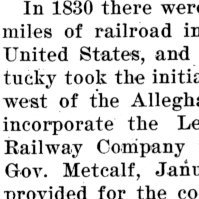
\includegraphics[width=\linewidth]{imagen3.jpg}
  \caption{Imagen 3.}\label{fig:awesome_image3}
\endminipage
\end{figure}


Para realizar las pruebas con imágenes, utilizamos los métodos de Umbral y Eliminación de Frecuencias Altas utilizando el mismo procedimiento que para señales unidimensionales alterando el código para que la matriz entera fuera procesada.\newline
Realizamos nuestras pruebas con los umbrales 5000, 10000 y 500000.\newline
Los resultados de las pruebas realizadas con el Umbral son las siguientes imágenes:\newline

\begin{figure}[H] % indico que voy a poner una figura y [h] indica que la posición relativa, tambien puedo usar t = top entre otros.
\hfill
\begin{minipage}[t]{.45\textwidth}
\begin{center}
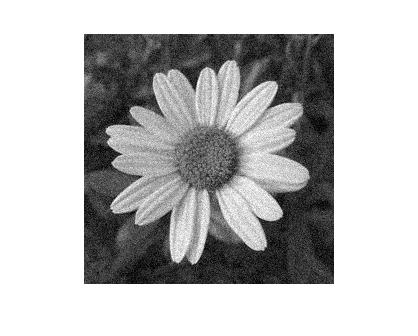
\epsfig{file=flor_ruido60_cota5000.jpg, scale=0.4} % primera imagen colocada a la izquierda
\caption{Imagen 1 con ruido de [-60, 60], umbral de 5.000.}
\label{fig-tc1}
\end{center}
\end{minipage}
\hfill
\begin{minipage}[t]{.45\textwidth}
\begin{center}
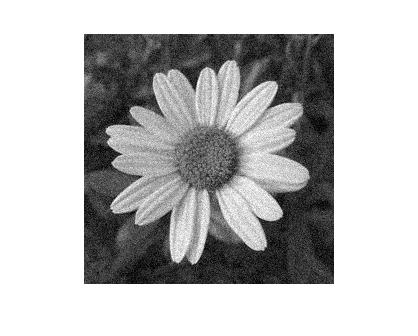
\epsfig{file=recu_flor_ruido60_cota5000.jpg, scale=0.4} % segunda imagen colocada a la derecha
\caption{Imagen 1 recuperada.}
\label{fig-tc2}
\end{center}
\end{minipage}
\hfill
\end{figure}


\begin{figure}[H] % indico que voy a poner una figura y [h] indica que la posición relativa, tambien puedo usar t = top entre otros.
\hfill
\begin{minipage}[t]{.45\textwidth}
\begin{center}
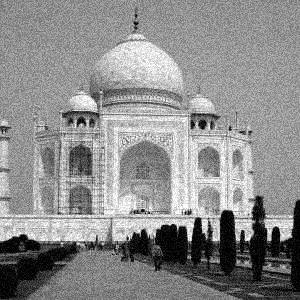
\epsfig{file=imagen2MasRuido.jpg, scale=0.4} % primera imagen colocada a la izquierda
\caption{Imagen 2 con ruido de [-25, 25], umbral de 500.000.}
\label{fig-tc1}
\end{center}
\end{minipage}
\hfill
\begin{minipage}[t]{.45\textwidth}
\begin{center}
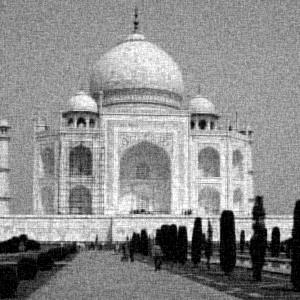
\epsfig{file=imagen2Restaurada.jpg, scale=0.4} % segunda imagen colocada a la derecha
\caption{Imagen 2 recuperada.}
\label{fig-tc2}
\end{center}
\end{minipage}
\hfill
\end{figure}

\begin{figure}[H] % indico que voy a poner una figura y [h] indica que la posición relativa, tambien puedo usar t = top entre otros.
\hfill
\begin{minipage}[t]{.45\textwidth}
\begin{center}
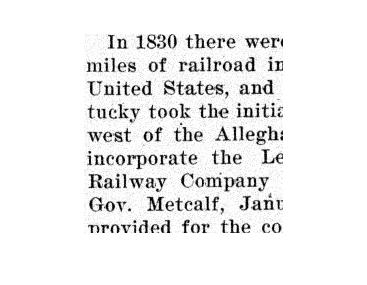
\epsfig{file=letra_ruido60_cota5000.jpg, scale=0.4} % primera imagen colocada a la izquierda
\caption{Imagen 3 con ruido de [-60, 60], umbral de 5.000.}
\label{fig-tc1}
\end{center}
\end{minipage}
\hfill
\begin{minipage}[t]{.45\textwidth}
\begin{center}
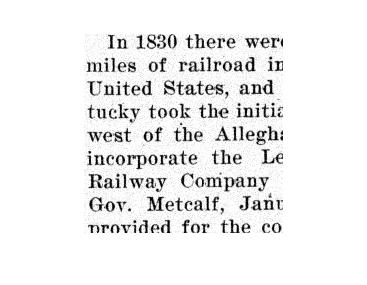
\epsfig{file=rec_letra_ruido60_cota5000.jpg, scale=0.4} % segunda imagen colocada a la derecha
\caption{Imagen 3 recuperada.}
\label{fig-tc2}
\end{center}
\end{minipage}
\hfill
\end{figure}


Los resultados de las pruebas realizadas con el método Eliminación de frecuencias altas son las siguientes imágenes:\newline

\begin{figure}[H] % indico que voy a poner una figura y [h] indica que la posición relativa, tambien puedo usar t = top entre otros.
\hfill
\begin{minipage}[t]{.45\textwidth}
\begin{center}
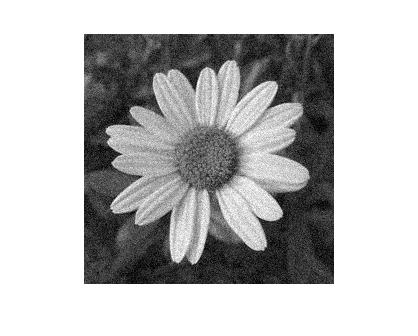
\epsfig{file=f2_flor_ruido60_cota10000.jpg, scale=0.4} % primera imagen colocada a la izquierda
\caption{Imagen 1 con ruido de [-60, 60], Eliminación de frecuencias altas de 10.000.}
\label{fig-tc1}
\end{center}
\end{minipage}
\hfill
\begin{minipage}[t]{.45\textwidth}
\begin{center}
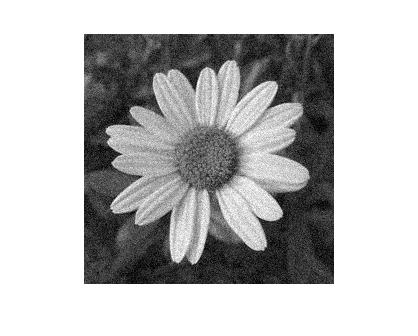
\epsfig{file=f2_recu_flor_ruido60_cota10000.jpg, scale=0.4} % segunda imagen colocada a la derecha
\caption{Imagen 1 recuperada.}
\label{fig-tc2}
\end{center}
\end{minipage}
\hfill
\end{figure}

\begin{figure}[H] % indico que voy a poner una figura y [h] indica que la posición relativa, tambien puedo usar t = top entre otros.
\hfill
\begin{minipage}[t]{.45\textwidth}
\begin{center}
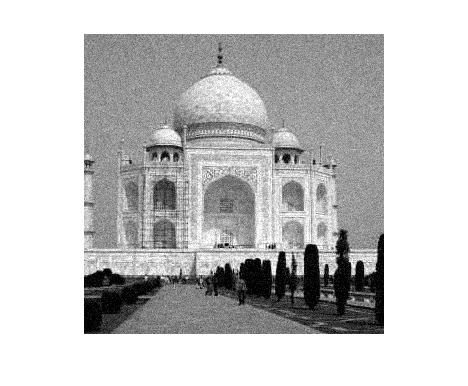
\epsfig{file=taj_ruido60_cota5000.jpg, scale=0.4} % primera imagen colocada a la izquierda
\caption{Imagen 2 con ruido de [-60, 60], Eliminación de frecuencias altas de 10.000.}
\label{fig-tc1}
\end{center}
\end{minipage}
\hfill
\begin{minipage}[t]{.45\textwidth}
\begin{center}
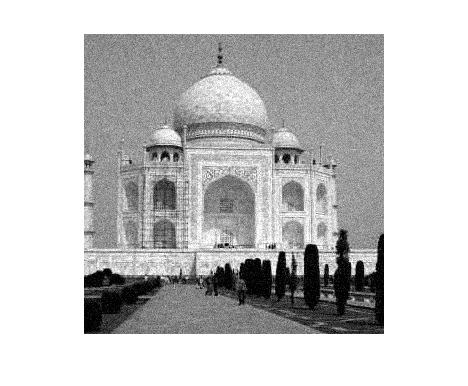
\epsfig{file=recu_taj_ruido60_cota5000.jpg, scale=0.4} % segunda imagen colocada a la derecha
\caption{Imagen 2 recuperada.}
\label{fig-tc2}
\end{center}
\end{minipage}
\hfill
\end{figure}

\begin{figure}[H] % indico que voy a poner una figura y [h] indica que la posición relativa, tambien puedo usar t = top entre otros.
\hfill
\begin{minipage}[t]{.45\textwidth}
\begin{center}
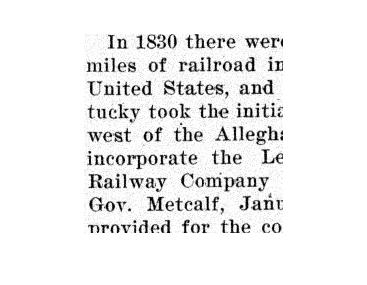
\epsfig{file=f2_letra_ruido60_cota10000.jpg, scale=0.4} % primera imagen colocada a la izquierda
\caption{Imagen 2 con ruido de [-60, 60], Eliminación de frecuencias altas de 10.000.}
\label{fig-tc1}
\end{center}
\end{minipage}
\hfill
\begin{minipage}[t]{.45\textwidth}
\begin{center}
\epsfig{file=f2_recu_letra_ruido60_cota10000.jpg, scale=0.4} % segunda imagen colocada a la derecha
\caption{Imagen 2 recuperada.}
\label{fig-tc2}
\end{center}
\end{minipage}
\hfill
\end{figure}

Por último, calculamos los distintos PSNR de cada imagen con ruido y su recuperada. Para exhibir los valores de manera clara, decidimos realizar gráficos en los que se muestra la diferencia entre el PSNR de la imagen+ruido y el PSNR de la recuperada. Los resultados fueron los siguientes:\newline


\begin{figure}[H] %[h] Aqui [b] para button [t] para top
\begin{center}
\includegraphics[width=300pt]{./imgsPX100k.jpg}
\caption[h]{PSNRs para una cota de 100.000.}
\end{center}
\end{figure}


\begin{figure}[H] %[h] Aqui [b] para button [t] para top
\begin{center}
\includegraphics[width=300pt]{./imgsPXY100k.jpg}
\caption[h]{Diferencias de PSNR's para una cota de 100.000.}
\end{center}
\end{figure}


\begin{figure}[H] %[h] Aqui [b] para button [t] para top
\begin{center}
\includegraphics[width=300pt]{./imgsPX300k.jpg}
\caption[h]{PSNR's para una cota de 300.000.}
\end{center}
\end{figure}


\begin{figure}[H] %[h] Aqui [b] para button [t] para top
\begin{center}
\includegraphics[width=300pt]{./imgsPXY300k.jpg}
\caption[h]{Diferencias de PSNR's para una cota de 300.000.}
\end{center}
\end{figure}


\begin{figure}[H] 
\begin{center}
\includegraphics[width=300pt]{./img3PXY100k.jpg}
\caption[h]{Diferencias de PSNRs para una cota de 100.000.}
\end{center}
\end{figure}

\begin{figure}[H]
\begin{center}
\includegraphics[width=300pt]{./img3PXY100k.jpg}
\caption[h]{Diferencias de PSNR's para una cota de 100.000.}
\end{center}
\end{figure}


\begin{figure}[H] 
\begin{center}
\includegraphics[width=300pt]{./img3PX300k.jpg}
\caption[h]{PSNR's para una cota de 300.000.}
\end{center}
\end{figure}


\begin{figure}[H] 
\begin{center}
\includegraphics[width=300pt]{./img3PXY300k.jpg}
\caption[h]{Diferencias de PSNR's para una cota de 300.000.}
\end{center}
\end{figure}


\section{Discusi\'on}
Al realizar el gráfico de comparación entre la DCT y la frecuencia original (que es una biyección), extrajimos nuestras conclusiones en base al coeficiente de magnitud. Cuando dicho valor es alto, podemos afirmar que el primer vector de la base está siendo multiplicado por un valor alto, por lo tanto, hay unas presencia del vector. Al observarlo en una nueva base, no podemos extraer conclusión alguna con respecto al tiempo, sólo podemos obtener información sobre la frecuencia.\newline
\newline
Tal como predicho en las secciones anteriores, pudimos observar, a partir de las DCT de las señales con ruido, que el agregado de ruido alteró levemente las señales sin deformarlas.\newline
\newline
Analizando los gráficos del 12 al 26, en el caso de señales unidimensionales, se puede ver que el valor del umbral es uno de los mayores determinantes a la hora de quitarle el ruido a una señal con dicho método. Por ejemplo, para la señal dopp1024, podemos concluir que los umbrales de 1000 y 3000 no filtran enormemente el ruido pero no deforman la señal al recuperarla. Contrariamente, los umbrales de 5000 y 10000 son altamente efectivos para quitarle el ruido a una señal pero son más propensos a deformarla.\newline
Por otro lado, en las señales referentes a g450, puede verse que el umbral más efectivo es el que tiene un valor de 5000. Si bien se pueden observar dos outliers que no se presentan en la señal original, la señal recuperada es la más aproximada a ésta.\newline
Por último, de acuerdo a los distintos umbrales utilizados para la señal ramp1234, podemos observar que el más conveniente resulta el valor 10000.\newline
\newline
A partir de los gráficos 27, 28 y 29, podemos concluir que cuando el ruido agregado excede el intervalo de [-20,20], la señal no puede recuperarse correctamente con el método umbral dando como resultado un PSNR menor al de la señal original con ruido. Esto ocurre pues las señales analizadas no se mueven en un rango de valores demasiado grandes por lo que el agregado de una gran cantidad de ruido lleva a la deformación de las mismas y a su dificultosa recuperación. Por otro lado, a menor ruido mayor recuperación. Esto nos permite afirmar que el método de umbral es muy eficiente siempre que la magnitud del ruido no supere en un 40\% los valores de la señal original independiente del rango o forma de la señal utilizada.\newline
\newline
En el caso del segundo método, podemos notar que los gráficos de recuperación de ruido (figuras 30, 31 y 32) no presentan una gran reducción del ruido, notamos que la cantidad de frecuencia suprimida no debía ser demasiado grande para no perder la información trascendente de la señal. Por otro lado, notamos que la cota a utilizar como tambien la cantidad de ruido a restar para lograr la mayor efectividad del método resultaba dependiente a cada tipo de señal y los valores entre los que éste se encontraba con lo cual el método permanece relativo a lo que se aplique. Por último, pudimos inferir, gracias a las distintas pruebas realizadas, que el método de 'Eliminación de frecuencias altas (interferencias) mediante filtrado de la señal' no es demasiado eficiente para quitar el ruido a señales que, por más de que haya una diferencia, ésta no resulta realmente notoria.

Para el caso de las señales bidimensionales, los resultados obtenidos a partir del primer método fueron que los umbrales debían hallarse en un rango que iba desde los 500.000 hasta los 8.000.000 db dependiendo del ruido. Al superar dicho valor, la imagen recuperada perdía definición mimetizándose de manera tal a que dejaran de distinguirse los elementos presentes en la misma.\newline
El umbral que mejor promedió según este algoritmo fue 3.000.000, dando como resultado un PSNR aproximado de 23 en la imagen restaurada para la mayoría de los casos.\newline
Por otra parte, observamos que una cota de 100.000 o menos podía arruinar la imagen en vez de mejorarla. Así como una cota chica podía no mejorar en nada a la imagen.\newline
Visualmente, puede notarse una leve mejoría en las imágenes recuperadas con el método umbral. El ruido ya no se ve como píxeles aislados unos de otros sino que la imagen se encuentra más límpida. Dicho resultado puede comprobarse con el incremento del PSNR visibles en las Figuras 51 a 58.
\newline
Dichos PSNR nos permitieron determinar que, si bien existe un umbral con mejor promedio de PSNR en la imagen recuperada, debe tenerse en cuenta que a menor cantidad de ruido menor debe ser la cota para lograr mayor eficacia.\newline
En el caso del segundo método, las imágenes recuperadas y las imágenes con ruido resultaron altamente similares. Si bien la mejora no es visual, ésta puede ser comprobada con los gráficos del PSNR (que se comportaron del mismo modo que para señales unidimensionales).\newline
\newline
%aca ponemos descripciones de los graficos, comparaciones, etc etc
Por lo tanto, podemos decir que, por un lado, para filtrar correctamente una señal (de una o dos dimensiones) la función y la cota de la misma deben estar estrechamente relacionadas con la cantidad y el tipo de ruido agregado. Para el caso del ruido, hemos intentado encontrar buenas cotas que resultaran buenas para la mayoría de los casos. Sin embargo, los resultados muestran que esto no siempre es suficiente. Algunas cotas que se comportan bien con la diferencia de PSNR (siendo el PSNR de la imagen restaurada mayor que el PSNR de la imagen con ruido) no presentan diferencias considerables, esto es, que la diferencia entre los dos PSNR es menor a 0.5.


\section{Conclusiones}
A modo de resumen, nuestro trabajo consistió en el agregado de ruido a señales unidimensionales y bidimensionales para que luego, éstas fueran recuperadas y volvieran lo máximo posible a su estado original. Para ello, utilizamos el método de Ruido Aditivo para agregar ruido y los métodos de Umbral y Eliminación de frecuencias altas mediante filtrado para ambos tipos de señales. Luego de una gran cantidad de pruebas, logramos encontrar resultados que efectivizaran los métodos otorgando señales más limpias de ruido y similares a las originales. Para el primer método, llegamos a la conclusión de que un umbral a partir de 800 mejora la señal cuando el ruido no exceda en valor al 40\% del valor más alto de la señal. Caso contrario, el método la distorsiona devolviendo una señal diferente a la deseada. Dichos resultados fueron verificados por el valor del PSNR de la señal con ruido y de la restaurada, que, cuando el ruido no era demasiado grande, marcaba mejorías de hasta 6 db.\newline
\newline
Por otro lado, el segundo método otorgó resultados que no reflejaron una gran mejoría en las señales (el PSNR resultó 0,20 db mayor que el de la señal con ruido). Sin embargo, dichas mejoras permanecieron lineales de acuerdo al aumento del ruido por lo que éste método resulta mejor que el primero en los casos en los que el ruido es demasiado grande.\newline
\newline
Nuestras conclusiones, en base a lo estudiado en las secciones anteriores, es que para lograr una señal bien filtrada con una función umbral, la cota debe ser elegida en función al tipo e intensidad del ruido. En nuestro caso, una gran cantidad de ruido aditivo no permite la correcta recuperación de la señal. Por otro lado, si el ruido agregado es menor que el umbral elegido, la funcion empeorará la señal. El análisis de los métodos mostró que la función umbral es efectiva para el ruido aditivo si la cota se encuentra cercana al promedio de ruido agregado. Por otro lado, el método de eliminación de frecuencias altas mostró no dar resultados demasiado eficientes, otorgando señales recuperadas altamente similares a las señales con ruido.

\section{Ap\'endices}
\subsection{A}
\begin{centering}
\large\bf Laboratorio de M\'etodos Num\'ericos - Primer Cuatrimestre 2013 \\
\large\bf Trabajo Pr\'actico N\'umero 2\\
\end{centering}

\vskip 1 cm
\hrule
\vskip 0.5 cm 

{\bf Introducci\'on}

La Transformada Discreta del Coseno  (DCT, por sus siglas en ingl\'es) es una herramienta que nos permite representar cualquier se\~nal en el plano de las frecuencias. Dado que es utilizada por el est\'andar de compresi\'on de im\'agenes JPEG y formato de video MPEG, se encuentra implementada en m\'as lugares de lo que pensamos: en cada c\'amara digital o tel\'efono m\'ovil. 
La DCT no solo tiene aplicaciones al mundo de la compresi\'on (donde los valores transformados pueden ser codificados de forma eficiente), sino tambi\'en al procesamiento: el an\'alisis de qu\'e frecuencias est\'an presentes en las se\~nales es esencial en ciertos contextos de aplicaci\'on.

La idea intuitiva de esta transformada, en el plano continuo, consiste en representar una funci\'on $f: \mathbb{R} \rightarrow \mathbb{R}$ en la base de funciones $\mathcal{B}=\{1, \cos(x), \cos(2x),...\}$.
En el plano discreto, la DCT se corresponde a un cambio de base: cada una de las funciones de la base $\mathcal{B}$ se discretiza en ciertos puntos pasando a ser una base de vectores en $\mathbb{R}^n$, (donde $n$ es la dimensi\'on del vector o se\~nal a transformar).
Es decir, dado un vector o se\~nal $x\in\mathbb{R}^n$ existe una matriz $M\in\mathbb{R}^{n\times n}$ de cambio de base que define la transformada DCT, donde $y=Mx$ es el vector o se\~nal transformado al espacio de frecuencias por la DCT (ver ap\'endice \ref{sec:dct}). Esta operaci\'on es f\'acilmente extensible a se\~nales de dos dimensiones (ver ap\'endice \ref{sec:dct2d}).


{\bf Enunciado}

El objetivo del trabajo es eliminar ruido sobre una se\~nal ruidosa $x\in\real^{n}$. Para ello se realiza el siguiente proceso: 
\begin{enumerate}
\item  $y:=Mx$ [Transformar usando Ec.~(\ref{eq:dctint}) de Ap. \ref{sec:dct}]
\item $\tilde{y} := f(y)$ [Modificar]
\item Resolver $M \tilde{x} = \tilde{y}$ [Reconstruir]
\end{enumerate}

 
Una forma de medir la calidad visual de la se\~nal reconstruida $\tilde{x}$, es a trav\'es del PSNR ({\em Peak Signal-to-Noise Ratio}).
EL PSNR es una m\'etrica `perceptual' (acorde a lo que perciben los humanos) y nos da una forma de medir la calidad de una imagen perturbada, siempre y cuando se cuente con la se\~nal original. 
Cuanto mayor es el PSNR, mayor es la calidad de la imagen. La unidad de medida es el decibel (db) y se considera que una diferencia de 0.5 db ya es notada por la vista humana. El PSNR se define como:
$$
\mathit{PSNR} = 10 \cdot \log_{10} \left( \frac{\mathit{MAX}^2_x}{\mathit{ECM}} \right)
$$
donde $\mathit{MAX}_x$ define el rango m\'aximo de la se\~nal (en caso de entradas de 8 bits sin signo, ser\'ia 255) y \emph{ECM} es el {\em error cuadr\'atico medio}, definido como:
$ \frac{1}{n} \sum_{i}{(x_{i} - \tilde{x}_{i})^2} $,
donde $n$ es la cantidad de elementos de la se\~nal, $x$ es la se\~nal original y $\tilde{x}$ es la se\~nal recuperada.

En la implementaci\'on realizada deben llevar a cabo los siguientes experimentos:
\begin{itemize}
\item Para varias se\~nales con distintos niveles de ruido, se deber\'an experimentar con al menos 2 estrategias (definiendo $f$ de forma conveniente) para modificar la se\~nal transformada $y$ (paso 2) con el objetivo de que la se\~nal recuperada $\tilde{x}$ contenga menos ruido; se deber\'an extraer conclusiones en cuanto a la calidad de la se\~nal recuperada, en funci\'on de la estrategia utilizada.
\item Se deber\'an repetir los anteriores experimentos tambi\'en sobre im\'agenes adaptando el m\'etodo para aplicar la transformada DCT en dos dimensiones seg\'un se explica en la ap\'endice \ref{sec:dct2d}. 
\item {\bf (Opcional)} Se deber\'a analizar la aplicaci\'on de la DCT `por bloques' sobre im\'agenes. Por ejemplo, si tenemos una imagen de $64\times 64$ p\'ixeles podemos subdividirla en: 4 bloques de $32\times 32$, o 16 bloques de $16\times 16$, o 64 bloques de $8\times 8$, y aplicar la DCT en 2D sobre cada uno de los bloques (considerar un tama\~no m\'inimo de $8\times 8$ para cada bloque).\\ 
Elegir una estrategia utilizada para se\~nales unidimiensionales y sacar conclusiones respondiendo a los siguientes interrogantes (realizando experimentos que justifiquen la respuesta): ?`Es lo mismo eliminar ruido sobre la imagen entera que de a bloques? ?`Qu\'e forma es m\'as conveniente en cuanto a la calidad visual? ?`Qu\'e forma es m\'as r\'apida? 
\end{itemize}

{\bf Formatos de archivos de entrada}

Las se\~nales ser\'an le\'idas de un archivo de texto en cuya primer l\'inea figuran la cantidad de datos y en la l\'inea siguiente se encuentran los datos en ASCII separados por espacios. Para leer y escribir im\'agenes sugerimos utilizar el formato {\em raw} binario \texttt{.pgm}\footnote{\url{http://netpbm.sourceforge.net/doc/pgm.html}}. 
El mismo es muy sencillo de implementar y compatible con muchos gestores de fotos\footnote{XnView \url{http://www.xnview.com/}} y Matlab.

\vskip 0.5 cm
\hrule
\vskip 0.1 cm

{\bf Fecha de entrega:} 
\begin{itemize}
\item \textsl{Formato electr\'onico:} jueves 16 de mayo de 2013, hasta las 23:59 hs., enviando el trabajo (informe+c\'odigo) a \texttt{metnum.lab@gmail.com}. El subject del email debe comenzar con el texto \verb|[TP2]| seguido de la lista de apellidos de los integrantes del grupo. 
\item \textsl{Formato f\'isico:} viernes 17 de mayo de 2013, de 18 a 20hs (en la clase del labo).
\end{itemize}

\newpage
\appendix
\section{Transformada Coseno Discreta}\label{sec:dct}

Para generar la matriz $M\in\real^{n\times n}$ que define la transformada de Coseno Discreta definimos: 
\begin{itemize}
 \item Vector de frecuencias:  $g = \left(\begin{array}{c} 0 \\ 1 \\ \vdots \\ n-1 \end{array} \right)$
 \item Vector de muestreo: $ s= {\displaystyle \frac{\pi}{n} }\left(\begin{array}{c} \frac{1}{2} \\1+\frac{1}{2} \\  \vdots \\ (n-1)+\frac{1}{2} \end{array} \right) $
 \item Constante de normalizaci\'on: $C(k) = \left\{ \begin{array}{lr}\sqrt{\frac{1}{n}} & k=1 \\ \sqrt{\frac{2}{n}} & k > 1 \end{array} \right.$
\end{itemize}

Siendo $T=\cos(g\cdot s^t)$ la matriz resultante de aplicarle el coseno a cada elemento de la matriz $g\cdot s^t$,
finalmente definimos, $\widehat{M}_{i,j} = C(i) \cdot T_{i,j}$

Para obtener una versi\'on entera de la transformaci\'on que define la matriz $M$, la cual ser\'a aplicada a se\~nales (o vectores) enteras en el rango $[0,q]$, definimos:
\begin{equation}
M = \left\lfloor \frac{q \widehat{M} + 1}{2}  \right\rfloor \label{eq:dctint}
\end{equation} 
donde $\left\lfloor\cdot\right\rfloor$ indica la parte entera inferior\footnote{El redondeo de un n\'umero $m$ pude definirse como $\lfloor m + 1/2 \rfloor$. Luego, $M$ se define como el redondeo de $\widehat{M}\cdot(q/2)$.}. (Es decir, escalamos los elementos de la matriz $M$ por $q/2$ y luego redondeamos los valores.)

\subsection{Extensi\'on a 2D}\label{sec:dct2d}
Dada una matriz $B\in\real^{n\times n}$, podemos extender f\'acilmente la transformada DCT a se\~nales de dos dimensiones. Para ello, aplicamos la transformaci\'on por filas y por columnas: $ M\, B\, M^t $

\end{itemize}
\subsection{B}

\large{\textbf{Implementaci\'on de nuestro programa:}}\newline

\centerline{\large{\textbf{main.cpp}}}

\lstloadlanguages{C++}
\lstset{language=C++,texcl=true,inputencoding=utf8/latin1,showstringspaces=false,
	frame=Ltb,
     framerule=0pt,
     aboveskip=0.5cm,
     framextopmargin=3pt,
     framexbottommargin=3pt,
     framexleftmargin=0.4cm,
     rulesep=.4pt,
    framesep=5pt,
basicstyle=\normalsize\ttfamily,
showstringspaces=false,
keywordstyle=\color{blue},
%identifierstyle=\ttfamily,
stringstyle=\color{Maroon},
commentstyle=\color{black},
rulecolor=\color{Gray},
xleftmargin=5pt,
xrightmargin=5pt,
aboveskip=\bigskipamount,
belowskip=\bigskipamount,
}

\lstinputlisting[language=C++]{main.cpp}

\centerline{\large{\textbf{tcd.cpp}}}
\lstinputlisting[language=C++]{tcd.cpp}

\centerline{\large{\textbf{tcd.h}}}
\lstinputlisting[language=C++]{tcd.h}

\section{Referencias}

%%un libro se referencia asi AUTOR. Año. Título; subtítulo. Edición. Lugar de publicación, editorial. Páginas o
%%volumen. (Serie comercial)

\begin{itemize}

\item BURDEN, RICHARD L. ; An\'alisis num\'erico, 7ma ed. 2002. M\'exico, Thomson Learning.

\item {http://planetmath.org/discretecosinetransform}

\item http://www4.ujaen.es/~satorres/practicas/practica2.pdf

\item http://www.eueti.uvigo.es/files/material\_docente/478/enmascaramiento.pdf

\end{itemize}

\end{document}
